\documentclass[10pt, a4paper, titlepage]{article}
\usepackage[utf8x]{inputenc}
\usepackage{ucs}
\usepackage{fullpage}
\usepackage{color}
\usepackage{index} % use index package to create indices
\newindex{todo}{tod}{tnd}{TODO List} % start todo list
\newindex{fixme}{fix}{fnd}{FIXME List} % start fixme list
\newcommand{\todo}[1]{\textcolor{blue}{TODO: #1}\index[todo]{#1}} % macro for todo entries
\newcommand{\fixme}[1]{\textcolor{red}{FIXME: #1}\index[fixme]{#1}} % macro for fixme entries
\usepackage{amsfonts}
\usepackage{pifont}
\usepackage{boxedminipage}
\usepackage{minitoc}
\usepackage{listings}
\usepackage{amsmath}
\usepackage{latexsym}
\usepackage{amsfonts}
\usepackage{amssymb}
\usepackage{wasysym}
\usepackage{graphicx}
\usepackage[T1]{fontenc}
\title{Automated Theorem Prover For Euler Diagrams \\ University of Brighton}
\author{Sasan Padidar}
\oddsidemargin 0.2in 
\begin{document}
\definecolor{CodeBackground}{rgb}{1.0,1.0,0.92}	
	
\lstset{ %
language=C++,                % choose the language of the code
basicstyle=\footnotesize,       % the size of the fonts that are used for the code
numbers=left,                   % where to put the line-numbers
numberstyle=\footnotesize,      % the size of the fonts that are used for the line-numbers
stepnumber=1,                   % the step between two line-numbers. If it's 1 each line will be numbered
numbersep=5pt,                  % how far the line-numbers are from the code
backgroundcolor=\color{CodeBackground},  % choose the background color. You must add \usepackage{color}
showspaces=false,               % show spaces adding particular underscores
showstringspaces=false,         % underline spaces within strings
showtabs=false,                 % show tabs within strings adding particular underscores
frame=single,			% adds a frame around the code
tabsize=4,			% sets default tabsize to 2 spaces
captionpos=b,			% sets the caption-position to bottom
breaklines=true,		% sets automatic line breaking
breakatwhitespace=false,	% sets if automatic breaks should only happen at whitespace
escapeinside={\%*}{*)}          % if you want to add a comment within your code
}

\maketitle

\begin{abstract}
Using visual modelling in specifying software is an ongoing research in mathematics and computer science. One of the important aims of visual modelling is to make it easier for people to produce software specification and allow them to reason about the specification using diagrammatic reasoning. Reasoning about diagrams is an error prone and time consuming task which also requires a certain amount of knowledge about diagrammatic reasoning, to be able to reason about the diagrams. In order to achieve the aim of making software specification easier for people, it is crucial to have automated systems that can perform most tasks automatically. In this project, the task of proving diagrams is automated by using a piece of software that automates the proving process of two diagrams. In this project all the processes that were involved in producing this piece of software are explained and the important aspects about the project that are related to computer science, software engineering and mathematics are discussed in detail. 
\end{abstract}
\newpage

~\vfill\begin{minipage}{\textwidth}  
\begin{LARGE}\textbf{Acknowledgements}\end{LARGE}\\\\


I would like to express my sincerest gratitude to my supervisors, without whom this project would not have been completed,

\begin{itemize}
\item Mr. Aidan Delaney
\item Dr. Gem Stapleton
\item Prof. John Howse 
\end{itemize}


for proposing the research criteria and also their invaluable advice, guidance and help throughout the course of this project. I am extremely thankful to them, for opening a new chapter in my understanding of software reliability, logic and academic research.\\

Also I would like to thank my parents for their support during my studies and providing me the opportunities to learn and grow. 


\end{minipage}\vfill~\newpage
\newpage
\tableofcontents
\linespread{1.3}
\large
\newpage


\newpage
\section{Introduction} 
\label{sec:introduction}

\subsection{Brief Introduction}
Using diagrams in a formal manner was described by \cite{Shin_1994} which made diagrams a useful tool that can be used for logical reasoning. The ability of using diagrams in a formalized manner makes it possible to produce software specification using diagrams as well. As a result of this, a great deal of work has been done on diagrammatic reasoning and visual modelling in the past few years to make this system more practical. \\
Software specification is very involved with logical statements and logical reasoning. For instance, if a designer wants to incorporate a constraint on a specific class or a function, he\footnote{He has to be read as he or she} has to write a logical statement to demonstrate that there is a constraint. Sometimes it is necessary to have these logical statements to be proved to be correct which requires an understanding of logical reasoning. The same kind of reasoning is also done in diagrammatic reasoning in a different manner. For example in diagrammatic logic it might be necessary to prove that two diagrams $ d_{1} $ and $ d_{2} $ (represented in figure (\ref{fig:d1demo}) and (\ref{fig:d2demo})) follow from one another.

\begin{figure}[h]
\begin{minipage}[h]{0.5\linewidth}
\centering
\includegraphics[scale=0.5]{images/d1.png}
\caption{$d_{1}$}
\label{fig:d1demo}
\end{minipage}
\hspace{0.5cm}
\begin{minipage}[h]{0.5\linewidth}
\centering
\includegraphics[scale=0.5]{images/d2.png}
\caption{$d_{2}$}
\label{fig:d2demo}
\end{minipage}
\end{figure}

In order to prove these diagrams, it it required to apply the unitary diagram proving algorithm, manually (for a novice user), as described in section \ref{unitary_algorithm}, However this algorithm could be implemented as a part of an automated prover to reduce errors that might occur, make the process faster and allow the user with no knowledge of the algorithm to be able to prove if the diagrams follow from each other. For example in this case $ d_{2} $ follows from $ d_{1} $ which means there is a logical proof from $ d_{1} $ to $ d_{2} $. This project's aim is to create a prover to be used in such circumstances.\\

In the project section \ref{sec:proj} detailed information about the project is given. In section  "Software Specification" \ref{sec:specification}, software specification is described.  The section "Visual Modelling" (\ref{sec:visual_modelling}) provides  all the necessary background knowledge about this project that was needed in order to be able to implement this project, is given. The "Design" section (\ref{sec:design}) provides all about the design process and what was learnt during the process. The "Implementation" section (\ref{sec:Implementation}) discusses the important aspects of the implementation of this project and the "Testing" section (\ref{sec:Testing}), is about how the program was tested.
 
\subsection{Introduction to Reliability}

Software reliability arguably is one of the most important issues in software engineering \cite{ANSI_91}. The idea of producing 100\% reliable software has been in computer science for a long time. According to ANSI (American National Standards Institute), Software Reliability is defined as: the probability of failure-free software operation for a specified period of time in a specified environment \cite{ANSI_91}. Although Software Reliability is defined as a probabilistic function, and comes with the notion of time, it must be noted that, it  differs from traditional “Hardware Reliability”, “Software Reliability” is not a direct function of time. Electronic and mechanical parts may become "old" and wear out with time and usage, but software will not wear-out during its life cycle. Software will not change over time unless intentionally changed. This makes software reliability a critical point in software production because software in many cases might last for a long period of time. Not being certain about the reliability of software will cause problems during the life cycle of the software and will have significant costs for its maintenance.  Therefore there are a great deal of benefits such as saving money over time or having more satisfied users, in producing reliable software both for the users and the designers.\\

In this day and age the importance of computer science is a widely accepted fact. One reason technology, specifically computer science, is significantly important is that all other sciences such as astronomy, physics and many other sciences depend on computers to be able to expand and improve themselves. Moreover, computers are one of the most remarkable tools which can be used to improve the quality of human life and take humanity to the next level of growth and expansion. This means in order to improve humanity and allow other sciences to grow and expand faster, computer science has to improve and expand. One of the major challenges that currently exists in computer science is providing reliable and cost effective software, fast. This means that producing reliable software is not an easy task right now which consequently means that, other sciences have problem in creating reliable software, fast, and concentrate more on their specialized field and spend their time and resources on solving their problem rather than spending their resources on creating reliable software. As a result of this the progress of evolution of other sciences and thus humanity cannot be as fast as it could be if creation of reliable software was cost-effective, easy and fast. Therefore having a structured, scientific and mathematical approach towards creating reliable software, fast, is inevitable in computer science. This improvement not only improves this science but allows other sciences to expand as the result of it. \\

This need for creating reliable software has led many mathematicians, computer scientists and software engineers to create new methods to properly specify and test software. There are a number of different approaches for specifying software in order to eliminate potential errors from the design and creating specific and non-ambiguous guidelines for creating functions. These methods have proven to be significantly helpful in creating reliable software and they are being used mainly on safety critical systems currently.


\subsection{Project Objectives}

This project aims to create an automated  prover for (Euler) diagrams which can prove the correctness of diagrams which, in the simplest explanation, means that the diagrams are logically sound and complete (that if a diagram is derived from another diagram, it follows the logical reasoning rules). This will make the process of specification much faster and less error prone.The aim of the project is creating a prover for unitary and compound diagrams. 

The advantages that this system has are:
\begin{enumerate}
\item This system will save the designer a lot of time in proving the correctness of the diagrams and allows the designer to spend more time on specification.
\item This system reduces the errors that might occur during the specification process because it can be used to prove the correctness of each step of the design rather than doing it when the specification is done.
\item The designer does not have to know the rules of diagrammatic proof. They can just use the prover to see whether diagrams follow from each other.
\end{enumerate}

Currently there is an automated theorem prover called “Edith” that is a unitary Euler diagram prover written in Java. Ideally, the ultimate goal of this project is to create another prover that is for compound diagrams as well as unitary which is open source and has a better structural design compared to Edith. But because this project is an experimental (research based) project, the decision of what path to take and what the final deliverable should be, will be decided during the development of the project. 


\newpage 
\section{Project}
\label{sec:proj}
This section is about the project from its beginning to its end. It discusses planning, objectives and final results.

\subsection{Objectives}
At the beginning of this project, the proposed topic was to create a prover for unitary diagrams and after the prover was developed and tested completely, then the decision about what direction the project should take would be decided. There were two directions the project could have taken:

\begin{itemize}
\item Expanding the unitary diagram prover.
\item Creating a compound diagram prover for compound diagrams.
\end{itemize}

The decision that was made, was to implement a compound diagram prover. Because this project is a research project, all the objectives were not set before starting the project which means the course of the project could have changed during the development process. The implications of this are discussed in the next sections. However, the exact objectives of the project that were decided on are listed below:

\begin{itemize}
\item Creating a unitary diagram prover for Euler diagrams.
\item "Ideally", creating a compound diagram prover for compound diagrams.
\end{itemize}

This means that the main objective of this project is creating a unitary diagram prover and then creating a compound diagram prover if there was enough time available.

\subsection{Required Knowledge}
To be able to plan and also design and implement such a system there are a number of subjects that have to be learnt before the start of the project. The required knowledge are:

\begin{itemize}
\item Understanding Euler diagrams
\item Unitary diagram proving algorithm
\item Understanding diagrammatic reasoning
\item Compound diagram proving algorithm
\item Practical object oriented design and analysis.
\end{itemize}

All the above subjects have to be learnt either before starting or in the course of the project to be able to design and implement this project. Learning about diagrams was done using the provided papers by the supervisors and learning about object oriented programming was done after a long research on designing in the course of the project.

\subsection{Planning}
As explained earlier the objective of the project at the beginning was to create a prover for unitary diagrams and then after it was done, deciding what path to take. Because of this, it was not possible to produce a plan for the entire project before starting it. Also because of lack of knowledge about the project and the processes that were involved, it was not possible to produce an accurate plan. Therefore a plan as it is normally expected of software projects was not produced initially. However, a plan was produced for the second part of the development of the compound theorem prover. The plan that was produced for the development of the unitary prover is provided below:\\

  
\begin{tabular}{| l | c | r | }
\hline
\multicolumn{3}{|c|}{Project Plan for Unitary Prover} \\
\hline	
  Understanding the requirement & Start from: 5/10/08 & To: 31/10/08 \\ \hline	
  Implementation of the Rules  & Start from: 5/10/08 & To: 31/10/08 \\ \hline	
  Implementing unitary prover algorithm & Start from: 1/11/08 & To: 30/11/08\\ \hline	
  Testing & Start from: 1/12/08 & To: 8/12/08\\ \hline	
  Writing the documentation & Start from: 30/11/08 & To: 6/12/08 \\
\hline	
\end{tabular}

Of course this plan did not work as it was supposed to, because when it was produced, there was no knowledge of what processes were going to be involved. So it was purely based on assumptions and guesses. For instance the testing and fixing the bugs, progressed until the beginning of January 2009 which means that the project was delayed for about a month. However for the second part of the project, it was more clear what processes were going to be involved and also there was an acceptable understanding of the requirements for the second part of the project. As a result of this, producing a more accurate plan for the second part of the project was a necessity before carrying on the research and development for creating a compound theorem prover. Therefore the plan that is represented in figure (\ref{fig:plan}) was produced with its corresponding Gantt chart.

\begin{figure}[]
\centering
\includegraphics[angle = 90, scale=0.55]{images/plan.png}
\caption{Second plan: For development of compound prover}
\label{fig:plan}
\end{figure} 

Asian, this plan also was inaccurate because of a number of reasons:

\begin{itemize}
\item Lack of understanding about software design which is explained in detail in section \ref{sec:design}.
\item The time that was needed for learning about the subject (diagrammatic reasoning mainly) took longer than expected.
\item Unforeseen problems that occurred with the programming language, namely problems with memory management (explained in more detail in section \ref{sec:Implementation}.
\item Misunderstanding a few points about visual modelling. The main cause of this issue was, unfamiliarity of using academic papers to learn a new subject. For example, learning the details about diagrams and diagrammatic reasoning requires reading a number of papers in a correct order to be able understand the subject. Not reading a paper or not knowing about just one simple point could lead to incorrect conclusions and therefore incorrect understanding. 
\item Significantly underestimating the time required for writing the project report. This single underestimation caused the entire plan to not work out as it was supposed to.
\end{itemize}

As it is clear, there were a great deal of issues in planning this project. It was extremely difficult to predict problems or perform risk analysis for this project. However, looking back on what was involved in this project, it was impossible to predict the issues that were going to happen and also producing a plan which could in fact be practical.\\


It is important to note that in the middle of the implementation of the project at the first of March, the implementation was stopped as the supervisors advice to stop the implementation and proceed to producing the project report. The time that was estimated for writing the documentation was significantly underestimated and that caused the planning to not work out. Although the requirements were understood and there was a relatively a good understanding of what should have been done for implementing the complete compound prover, lack of time did not allow the compound prover to be completed.
  
\subsection{Time Management}

Both the research and development of this project consumed a great deal of time which was not expected in the magnitude that it did. On average at least 40-50 hours was spent on this project each week (for both research and development). The way the time was spent on this project might have been more than necessary but because of the amount of learning that was involved in better understanding of visual modelling, diagrammatic reasoning, logic and software design it seems to be acceptable. On the whole, it is true that the planning did not work but the way that the time was spent was not the cause of the failure of the plans.
    
\subsection{Tasks}

The table below shows the tasks that were involved in this project and it shows which ones of them were completed.\\


\begin{tabular}{| l | c | }
\hline
\multicolumn{2}{|c|}{Tasks} \\
\hline	
  Implementation of Restrictive reasoning rules & Completed\\ \hline	
  Implementation of Unitary diagram theorem prover algorithm & Completed\\ \hline	
  Implementation of Compound diagram structure & Completed\\ \hline	
  Implementation of Applying compound diagram rules & Completed\\ \hline
  Implementation of Compound diagram prover & Not Completed\\ \hline	
\end{tabular}

Although the compound prover was not completed, the ability to be able to apply rules was designed and incorporated in the program.

\section{Software Specification}
\label{sec:specification}

The aim of software specification is to create a (high-level) model serving to specify an abstract architecture for the required system where its outcome must be understood \cite{Howse_2005}. 

Producing reliable software in non-safety critical systems should be as important as safety critical systems because these systems are going to exists usually for a long period of time and need to function as expected in that period of time. This reduces maintenance cost and also makes users more satisfied. In order to have very reliable software there must be a clear detailed specification for the entire system. There also has to be a set of defined metrics for creating software because by using these metrics, it will be possible to measure the reliability of a piece of software and then take action accordingly. The set of metrics must clearly specify the expectation boundary and the absolute purpose of the software. Also there should exist a system that can ensure the reliability of the software automatically because if the current methods evolve to a more complex method they will discourage engineers to use them as it will make their job (production of reliable software) even more complex and expensive because of the added workload to the project. 


\subsection{Formal Languages}

Software specification can be written using a number of formal languages such as ML. A formal language is a set of words i.e. finite strings of letters or symbols \cite{Mateescu_1997}. By using the words and symbols it is possible to represent different operations which can be used for specifying a particular operation.\\

Formal languages use some symbols such as $\vee, \wedge, \in, \lambda$ to describe different parts of the system. This is just for demonstrating what symbols are included in symbolic logic, there are many more symbols as well.

\subsection{Visual Modelling}
 
As stated in the “formal languages” section using formal languages is generally difficult and they are hard to read. This has led to a number of researchers (mainly mathematicians) to look for an easier method of specifying software which offers the same level of formalism and accuracy as formal languages do. The result of this research is using visual modelling namely diagrammatic modelling, rather than symbolic modelling. Research that is currently being carried out on use of diagrams for  software specification is producing some promising tools that can be used to specify software formally. This method of specification uses diagrams, mainly Euler/Venn diagrams to represent different aspects of  the system that is being specified and, then. by applying diagrammatic reasoning rules to each diagram the specification can be proved to be correct. For example in a specification for a library system, the requirement might have a constraint that "there exists some films in the library" ($ Film \cap Library \neq \emptyset $)  represented in figure (\ref{fig:lib1}) and in a particular state of the program there is no films available in the library ($ Film \cap Library = \emptyset $) as respresented in figure(\ref{fig:lib2}). Using diagrammatic reasoning it is not "logical" to be able to reach diagram $ d_{2} $ from $ d_{1} $. Which means that proving that the diagram provided in figure(\ref{fig:lib2}) follows from the diagram provided in figure (\ref{fig:lib1}) is not possible using the unitary diagram proving algorithm. Therefore the constraint that was imposed on this system that the library has some films has failed which means that the specification is not logically sound and complete.

\begin{figure}[h]
\begin{minipage}[h]{0.5\linewidth}
\centering
\includegraphics[scale=0.7]{images/library1.png}
\caption{$d_{1}$}
\label{fig:lib1}
\end{minipage}
\hspace{0.5cm}
\begin{minipage}[h]{0.5\linewidth}
\centering
\includegraphics[scale=0.7]{images/library2.png}
\caption{$d_{2}$}
\label{fig:lib2}
\end{minipage}
\end{figure}

 
This system has a number of possible advantages which include:
\begin{enumerate}
\item Specification can be understood more easily by looking at a number diagrams rather than reading the symbolic statements that other languages use. For instance the diagram provided in figure (\ref{fig:lib2}) can be interpreted as $ Books \cap Library \neq \emptyset $  or $ Library \cap Film = \emptyset$. However, by just a simple glance at the diagram both given logical statements can be understood without reading a single statement. 
\item Reading and understanding the specification becomes faster than using symbolic statements because a picture can say a great deal more compared to a single logical statement .
\item It is significantly easier and faster to produce the specification using diagrams rather than using the symbols.
\end{enumerate}

This makes specification relatively easier and faster which is quite a compelling reason for choosing diagrammatic notation as the specification method as the engineers are after an easier and faster specification method. These advantages are all arguable, they should not be treated as proven facts and they are not the only advantages of the diagrammatic system. Different designers and engineers require different tools in order to produce their specification. It is a scientific fact that different people learn and conceive information in different manners. Some people learn visually faster and can remember information visually and this system is just another tool that has to exist for people who are more comfortable with visual information. This diagrammatic system is still being developed and there is a great deal left to be discovered in this area. It is too early to judge whether the diagrammatic system has any particular advantages over symbolic logic and it is difficult to have a compelling scientific fact for designers in symbolic logic to adopt diagrammatic system and use that for their specification work. However it seems that the diagrammatic system and symbolic logic have to coexist to make an efficient specification method. For a more detailed information on diagrammatic system refer to \cite{Aidan_Gem}.\\
   
As explained above in order to use the diagrammatic method it is needed to apply diagrammatic reasoning rules to diagrams to ensure that the specification is correct logically. This means that the designer has to apply rules to each diagram that is supposed to follow from another diagram and prove that the meaning the diagrams imply is correct logically (will be explained in more detail). This is currently done manually by the designers which is error prone and is a tedious process. For instance when a designer has specified what should happen after an event in the program has occurred, he has to represent the starting state of the program in a diagram and also the desired state after the event has occurred. Then by applying reasoning rules that the diagrammatic system provides he can prove whether the diagrams truly follow from one another logically. If not that means the specification has errors in it and therefore the program that is written based on that specification has bugs in it (only if the program conforms to the specification). \\


\newpage

\section{Visual Modelling}
\label{sec:visual_modelling}

\subsection{Brief Diagrams History}
After Shin's \cite{Shin_1994} work on demonstrating that it is possible to have a sound and complete diagrammatic logic, diagrams have become a valuable tool to be used in logic. One of the most important reasons that diagrams are used is because they are much more intuitive to understand compare to symbolic logic. Understanding and using symbolic logic needs the ability to understand and formulate rigorous arguments. As a result of this issue symbolic logic is not accessible to a wide range of users i.e. software engineers, programmers, computer scientists, etc. Software Engineers are used to the idea of using frameworks such as testing or designing (like patterns) frameworks that are standard in the industry which they can be used to communicate with other software engineers in a standard way. Having symbolic logic as a framework is just inefficient because of the vast amount of knowledge engineers should have in order to understand  the rigorous arguments and logical statements. Moreover experience has proven that software engineers are more comfortable with visual modelling tools such as the Unified Modelling Language (UML) because of thier, relatively, user friendliness. Considering these facts it seems compelling that there is a need of a diagrammatic system that can represent logical statements. This diagrammatic system has the potential to become the standard modelling framework in the industry and could be beneficial to many potential users due to its rather straightforward, intuitive way of understanding it \cite{Gem_1}.
Figure 1 below demonstrates the difference between understanding the meaning of a diagram compared to a symbolic statement. The diagram below can be interpreted in different ways. An interpretation of it could be “There does not exist any car that is a computer or a PC” in symbolic logic it is:
$$ \neg\exists x ((Computer(x) \vee pc(x)) \wedge Car(x))$$
\begin{figure}[h]
\centering
\includegraphics{images/diag2_21.png}
\caption{An Euler Digram}
\end{figure}

\begin{figure}[h]
\centering
\includegraphics{images/diag2_22.png}
\caption{The normal form of the diagram}
\end{figure}

The shaded areas represent emptiness. The normal form and the shading are explained in later.

\subsection{Overview Of Diagrams}
There a number of different diagrams that are used by mathematicians in the area of logic that are related to sets i.e. Venn diagrams, Euler diagrams, Spider diagrams, Johnston diagrams, etcetera. These diagrams all have some advantages and disadvantages in different circumstances. Euler diagrams are the main concern here as this project is about implementing a prover for Euler diagrams. 

\subsection{Euler Diagrams}

The definition of Euler diagrams as described in \cite{Fish_2007} is Euler diagrams are finite collections of simple closed curves (shapes that do not self-intersect) drawn in the plane and may also contain shading. Euler diagrams consist of contours and zones. The definitions regarding Euler diagrams are:
\begin{itemize}
\item A Contour is a closed curve that represents a set. For instance in the diagram below “A” is a contour.
\item A Zone is a region in the plane that is inside cetain contours and outside the rest. 
\item A Shaded Zone in Euler diagrams means that the specific area in the diagram is empty. In other words the shaded zone means there is no element in that area.
\item A Zonal Region is a region that becomes a zone when contours are removed. 
\end{itemize}
For more detail refer to \cite{Fish_2007}.

The diagram below is an example of an Euler diagram.

\begin{figure}[h]
\centering
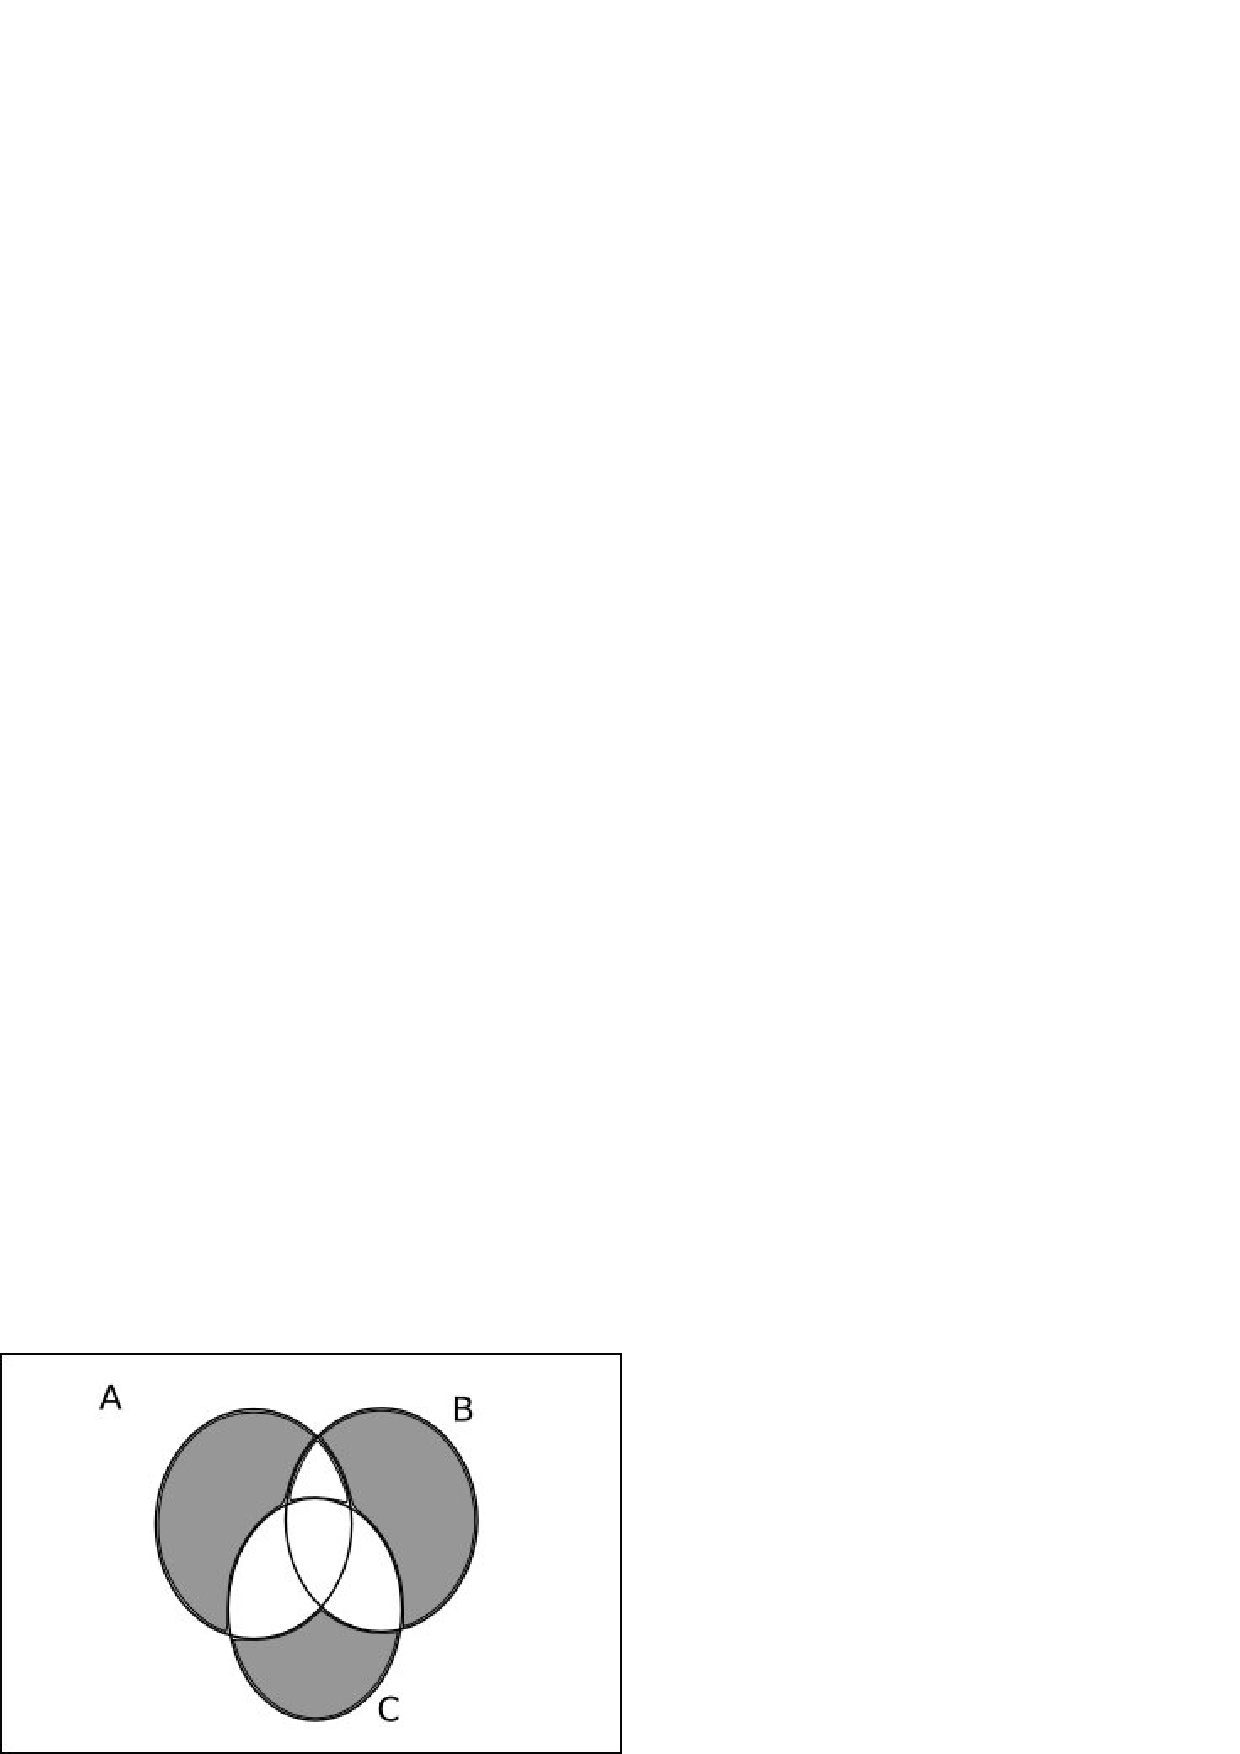
\includegraphics{images/dia2.png}
\caption{An Euler Diagram}
\end{figure}

There might be a slight confusion between Euler diagrams and Venn diagrams because of their similarities. Venn diagrams can be seen as a special case of Euler diagrams, as Venn diagrams must contain all possible zones, whereas Euler diagrams can contain a subset of all possible zones. In Venn diagrams a shaded zone represents an empty set, whereas in an Euler diagram the corresponding zone could be missing from the diagram. This means that as the number of contours increase, Euler diagrams are typically less visually complex than the equivalent Venn diagram, particularly if the number of non-empty intersections is small \cite{Kent_Euler}.

The intersection of the contours in Euler diagrams means that there might exist common elements between those particular contours which represent sets. Each Euler diagram has an abstract syntax which describes the diagram using text. This abstract syntax helps significantly in creation of an automated theorem prover for the diagrams because it provides a structured framework to be used in describing each diagram while trying to prove theorems (this will be explained in the later chapters). To give an example of the abstract syntax, the abstract syntax of the above diagram is written below.
\newline \newline
$contours =  \lbrace A, B, C \rbrace $ \newline
$zones = \lbrace (A , BC) , (B , AC), (C, AB), (AB , C) , (BC , A) , (AC, B), (ABC , ), ( \emptyset  , ABC) \rbrace  $ \newline 
$shaded zones = \lbrace (A , BC), (B , AC) , (C, AB) \rbrace  $ \newline

The abstract syntax of the diagram only puts the diagram in textual format and says nothing else about it. It is still possible to read the abstract syntax as reading the diagram itself. For instance the zone $(A, BC)$ can be read as inside $A$ and outside $B$ and $C$. Zones are put into brackets in the abstract form and the separating comma separates the inside of the zone with its outside. To clarify, the contour label(s) on the right side of the comma are the part of the zone that is being considered but just having that is not enough because the contour(s) might have intersections with other contours that are not being considered. Therefore it is necessary to state on the left side of the comma what contours are not included in the zone.

\subsection{Diagrams}
There are two types of diagrams in this system:
\begin{itemize}
\item Unitary Diagrams: A unitary diagram is just a single (Euler) diagram which is constructed without the use of any operators.
\item Compound Diagrams: A compound diagram is a diagram that is constructed using the operators $\wedge$ or $\vee$ or both. The operator $\neg$ can also be used to represent the complement of a diagram.
\end{itemize}


\subsection{Notations}
The notations that are used in this system are explained below:

\begin{itemize}
\item $ \vee : $ This operator is called the "Or" operator.   \\
\item $ \wedge : $ This operator is called the "And" operator.  \\
\item $ \neg : $ This operator is called the "Not" operator. It is used to represent the negation of its operand (a diagram). \\
\item $ \leftrightarrow : $ This operator means that starting from the left side it is possible to reach the conclusion on the right side or starting from the right side it is possible to reach the conclusion on the left side. It means that the statement that has this operator in, is correct both ways. \\
\end{itemize}

For details about different operators and understating set theory refer to \cite{Taylor_book}

\subsection{Reasoning}

In order to have a formal diagrammatic system it is necessary to have a set of well defined rules that can be used to prove the correctness of diagrams (that the diagrams are sound and complete which means they follow all logic behind diagrammatic reasoning) formally. Because of this reason a number of well defined rules are defined in a number of different papers which include \cite{Fish_2007} and \cite{Gem_Judith}. These rules are significantly helpful in structuring the process of proving (explained in later sections). By substituting different diagrams in different reasoning rules it is possible to prove certain issues about that diagram or diagrams. This depends on the context in which the diagrams are being considered. For this project a certain number of rules are used to check if there exists a proof between two diagrams. In this project the so-called restrictive reasoning rules are used. It is possible to weaken these rules and have a number of different rules called the “relaxed reasoning system” \cite{Fish_2007}. The reason that restrictive reasoning rules are used in this project is because the ultimate goal of the project is to implement a prover for compound diagrams which does not require the relaxed reasoning rules to be completed.  

\subsection{Reasoning Rules}
The rules that are used in the prover are :
\begin{enumerate}
\item Add Contour
\item Remove Contour
\item Add Shaded Zone
\item Remove Shaded Zone
\item Identity Law
\item Complement Laws
\item De Morgan's Laws
\item Involution
\item Distributivity
\item Idempotency 
\item Inconsistency
\item Connecting a diagram
\item Removing a diagram
\end{enumerate}

Each rule is explained with examples below in detail.

\subsubsection{Add Contour}
This rule simply adds a new contour to the diagram. Provided that the contour is not already in the diagram. Adding the contour causes each zone to be split into two zones (one inside and one outside the new contour), and shading is preserved \cite{Fish_2007}.
The figures below demonstrates how a new contour is added.
As it is clearly visible the new contour $ C $ is added to the diagram and has split all zones into two zones. The abstract syntax of figure \ref{fig:add1} before adding is:\newline
$contours =  \lbrace A, B \rbrace $ \newline
$zones = \lbrace (A , B) , (B , A), (AB , \emptyset) , (\emptyset , AB) \rbrace  $ \newline 
$shaded zones = \lbrace (AB , \emptyset) \rbrace  $ \newline

\begin{figure}[h]
\begin{minipage}[h]{0.5\linewidth}
\centering
\includegraphics[scale=0.5]{images/diag3add1.png}
\caption{Before applying Add contour}
\label{fig:add1}
\end{minipage}
\hspace{0.5cm}
\begin{minipage}[h]{0.5\linewidth}
\centering
\includegraphics[scale=0.5]{images/diag3add2.png}
\caption{After applying Add contour}
\label{fig:add2}
\end{minipage}
\end{figure}

After adding the new contour the abstract syntax becomes:\newline
$contours =  \lbrace A, B, C \rbrace $ \newline
$zones = \lbrace (A , BC) , (B , AC), (C, AB), (AB , C) , (BC , A) , (AC, B), (ABC , ), (  , ABC) \rbrace  $ \newline 
$shaded zones = \lbrace (AB , C), (ABC , ) \rbrace  $ \newline

\subsubsection{Remove Contour}
Removing a contour is the reverse process of adding a contour. All the zones that are involved with that contour will combine with other zones to form a single zone. For all pairs of zones that have to combine in order to form a single zone which either both shaded or both nonshaded, the shading is preserved and no new shading is added.\cite{Fish_2007}. In the abstract syntax all the zones that are created by the add contour rule must be removed and all the zones that have the contour label that is being removed must be modified to exclude the contour label.

The diagrams below demonstrate removing of contour $C$. The abstract syntax of figure \ref{fig:add3} before removing the contour is:\newline
$contours =  \lbrace A, B, C \rbrace $ \newline
$zones = \lbrace (A , BC) , (B , AC), (C, AB), (AB , C) , (BC , A) , (AC, B), (ABC ,\emptyset ), (\emptyset  , ABC) \rbrace  $ \newline 
$shaded zones = \lbrace (AB , C), (ABC , \emptyset) \rbrace  $ \newline

\begin{figure}[h]
\begin{minipage}[h]{0.5\linewidth}
\centering
\includegraphics[scale=0.5]{images/diag3add2.png}
\caption{Before applying remove contour}
\label{fig:add3}
\end{minipage}
\hspace{0.5cm}
\begin{minipage}[h]{0.5\linewidth}
\centering
\includegraphics[scale=0.5]{images/diag3add1.png}
\caption{After applying remove contour}
\label{fig:add4}
\end{minipage}
\end{figure}

After removing contour:\newline
$contours =  \lbrace A, B \rbrace $ \newline
$zones = \lbrace (A , B) , (B , A), (AB , ) , ( , AB) \rbrace  $ \newline 
$shaded zones = \lbrace (AB , ) \rbrace  $ \newline

\subsubsection{Add Shaded Zone}

Adding a shaded zone adds a missing zone to the diagram and shades it. To clarify, there are situations that by just looking at the diagram it is not possible to see all the zones. It is necessary at times (i.e. for proving) to present the diagram in a way that all zones are visible. The "invisible" (missing) zones can be added to the diagram by this rule and because they are not visible it means they are empty and therefore they have to be shaded. However the new diagram that is created as the result of adding the new missing zone is different from the starting diagram but has a strong relationship with it  i.e. it contains the same zones plus a new zone and the same shaded zones plus that new zone shaded. If a missing zone is added but it is not shaded the new diagram will not be the same as the starting diagram. A missing zone means that the zone is not in the diagram (which in symbolic logic means the set is empty) and is not considered to have any elements in it. Adding the missing zone and not shading it means the diagram is modified and does not have a strong relationship with the starting diagram. \newline

The abstract syntax before adding the missing zones represented in figure \ref{fig:missing1}.\newline
$contours =  \lbrace A, B, C \rbrace $ \newline
$zones = \lbrace (A , BC) , (B , AC), (AB , C) , (AC, B), (  , ABC) \rbrace  $ \newline 
$shaded zones = \lbrace \rbrace  $ \newline

\begin{figure}[h]
\begin{minipage}[h]{0.5\linewidth}
\centering
\includegraphics[scale=0.5]{images/d4sh1.png}
\caption{Before applying add shaded zone}
\label{fig:missing1}
\end{minipage}
\hspace{0.5cm}
\begin{minipage}[h]{0.5\linewidth}
\centering
\includegraphics[scale=0.5]{images/d4sh2.png}
\caption{After applying add shaded zone (three times to add all missing zones)}
\label{fig:missing2}
\end{minipage}
\end{figure}

After adding the missing zones and shading it represented in figure \ref{fig:missing2}. Note that this rule  is used three times to ad all missig zones to the diagram.\newline
$contours =  \lbrace A, B, C \rbrace $ \newline
$zones = \lbrace (A , BC) , (B , AC), (C, AB), (AB , C) , (BC , A) , (AC, B), (ABC , ), (  , ABC) \rbrace  $ \newline 
$shaded zones = \lbrace (C, AB), (BC , A), (ABC , ) \rbrace  $ \newline

As it is clearly visible in the diagrams, the zones $(C, AB) , (BC, A), (ABC, )$ were not mentioned in the abstract syntax of figure \ref{fig:missing1} and by looking at the diagram (in figure \ref{fig:missing2}) it is obvious that the zones are missing while the diagram implies that those zones exist.

\subsubsection{Remove Shading from a Zone}

This rule is the reverse of the add shaded zone rule. A shaded zone can be removed but only if there is at least one zone inside each contour in the resulting diagram and the zone outside all the contours remains \cite{Fish_2007}. If a missing zone is added to a diagram (which is shaded) is no longer needed to be shaded i.e. it contains some elements in it, it is possible to remove the shading from the zone by applying this rule. 
\\

Abstract syntax of figure \ref{fig:d5empty}\newline
$contours =  \lbrace A, B \rbrace $ \newline
$zones = \lbrace (A , B) , (B , A), (AB , \emptyset) , (\emptyset , AB) \rbrace  $ \newline 
$shaded zones = \lbrace (AB , \emptyset) \rbrace  $ \newline

\begin{figure}[h]
\begin{minipage}[h]{0.5\linewidth}
\centering
\includegraphics[scale=0.5]{images/diag3add1.png}
\caption{Before removing shaded zone}
\label{fig:d5empty}
\end{minipage}
\hspace{0.5cm}
\begin{minipage}[h]{0.5\linewidth}
\centering
\includegraphics[scale=0.5]{images/d5.png}
\caption{After removing shaded zone}
\label{fig:d5}
\end{minipage}
\end{figure}


Abstract syntax of figure \ref{fig:d5}\newline
$contours =  \lbrace A, B \rbrace $ \newline
$zones = \lbrace (A , B) , (B , A), (AB , ) , ( , AB) \rbrace  $ \newline 
$shaded zones = \lbrace \rbrace  $ \newline

As it is visible the shading is removed from the zone in figure \ref{fig:d5} and now it means that zone $ (AB, C) $ is not empty any more or "might" contain one or more elements in it but note that Euler diagrams do not say anything about non-emptiness of zones they can only talk about about the emptiness of zones.

\subsubsection{Identity Law}
Identity law says a diagram connected to another empty diagram by an "and ($ \wedge $)" operator is equivalent to the diagram itself and vice versa. 
$$ d_{1} \wedge \square \longleftrightarrow d_{1}$$

\subsubsection{Complement Laws} 
The complement laws in diagrammatic logic are:
$$ d_{1} \vee \neg d_{1} \longleftrightarrow \square $$
and
$$ d_{1} \wedge \neg d_{1} \longleftrightarrow \neg  \square $$

\begin{figure}[h]
\begin{minipage}[h]{0.5\linewidth}
\centering
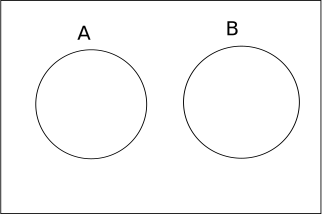
\includegraphics[scale=0.5]{images/d7-1.png}
\caption{$ d_{1} $}
\label{fig:d7}
\end{minipage}
\hspace{0.5cm}
\begin{minipage}[h]{0.5\linewidth}
\centering
\includegraphics[scale=0.5]{images/d7-2.png}
\caption{$ \neg d_{1} $}
\label{fig:d7-1}
\end{minipage}
\end{figure}

In the above diagram in figure \ref{fig:d7}, $ A \cap B = \emptyset $  and in the diagram in figure \ref{fig:d7-1}, $ A \cap B  = \emptyset $. So $ ( A \cap B ) $ or $ ( A \cap B )  = \emptyset $. This is meant by $ d_{1} \vee \neg d_{1} $ in the above law. Also in $\neg d_{1}$, $ A \cap B \neq \emptyset $ (it is possible to assert this because of the $ \neg $ operator before $ d _{1}$). Therefore $ ( A \cap B ) $ and $ ( A \cap B ) \neq \emptyset $. This is also is meant by $ d_{1} \wedge \neg d_{1} $.\\

Note that the reverse of this law is also correct which is represented by $\longleftrightarrow$.  

\subsubsection{De Morgan's Laws}
These laws say that if a compound diagram is neglected and the connector between the diagrams is a $\vee$ operator is the same as the complement of the first diagram connected with a $\wedge$ and the complement of the second diagram. Also if a compound diagram is neglected and the connector between the diagrams is a $\wedge$ operator is the same as the complement of the first diagram connected with a $\vee$ and the complement of the second diagram.
$$ \neg(d_{1} \vee d_{2}) \longleftrightarrow \neg d_{1} \wedge \neg d_{2} $$

$$ \neg(d_{1} \wedge d_{2}) \longleftrightarrow \neg d_{1} \vee \neg d_{2} $$

In the compound diagram in figure \ref{d8}, $ d_{1} $ says that  $ B \subseteq A $ and $ d_{2} $ says that $ A \cap C = \emptyset $. Considering $ \neg (d_{1} \wedge d_{2}) $, $ d_{1} \wedge d_{2} $ says that $ B \subseteq A$ and $A \cap C = \emptyset $. Also $ \neg (d_{1} \wedge d_{2}) $ says that $ B \nsubseteq A $ or $ A \cap C \neq \emptyset $ but this is what $ \neg d_{1} \vee \neg d_{2} $ tells us. 

\begin{figure}[h]
\centering
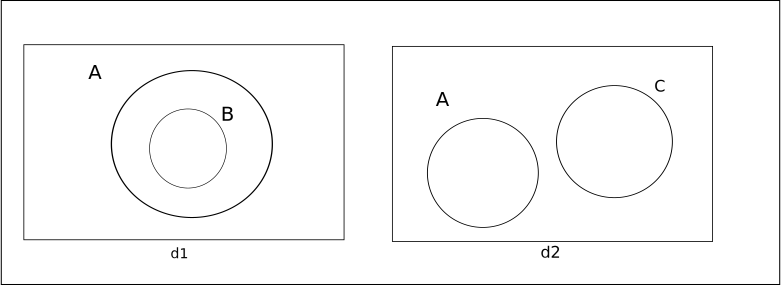
\includegraphics[scale=0.7]{images/d8.png}
\caption{De Morgan's Law}
\label{d8}
\end{figure}

\subsubsection{Involution}

This rule states 
$$ \neg \neg d_{1} \longleftrightarrow d_{1} $$
which means that the complement of a complement is the diagram itself.

\subsection{Distributivity}
The distributivity rule is
$$ d_{1} \wedge (d_{2} \vee d_{3}) \longleftrightarrow (d_{1} \wedge d_{2}) \vee (d_{1} \wedge d_{3}) $$
$$ d_{1} \vee (d_{2} \wedge d_{3}) \longleftrightarrow (d_{1} \vee d_{2}) \wedge (d_{1} \vee d_{3}) $$


\begin{figure}[h]
\centering
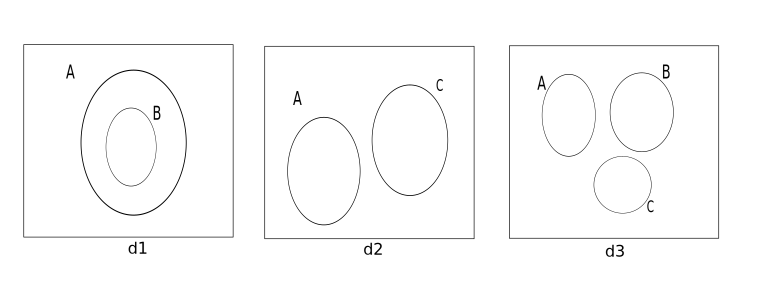
\includegraphics[scale=0.7]{images/d9.png}
\caption{Distributivity Rule Example}
\label{d9}
\end{figure}

Consider the diagrams represented in figure \ref{d9}, the diagram $ d_{1} $ tells us that $ B \subseteq A $, $ d_{2} $ tells us that $ A \cap C \neq \emptyset $ and $ d_{3} $ tells us that $ A \cap B \cap C = \emptyset $. Consider $ d_{1} \wedge (d_{2} \vee d_{3}) $, $ (d_{2} \vee d_{3}) $ says that $ A \cap C \neq \emptyset $ or $ A \cap B \cap C = \emptyset $ and $ d_{1} $ tells us that $ B \subseteq A $. However, $ B \subseteq A $ and $ A \cap C \neq \emptyset $ or $ A \cap B \cap C = \emptyset $ is also meant by $ (d_{1} \wedge d_{2}) \vee (d_{1} \wedge d_{3}) $. 


\subsection{Idempotency}
Any diagram connected to itself by an "or" or "and" connector is equivalent to the diagram itself. 
$$ d_{1} \longleftrightarrow d_{1} \wedge d_{1} $$
$$ d_{1} \longleftrightarrow d_{1} \vee d_{1} $$

\subsection{Information Weakening Rules}
Information weakening rules weaken (or make more general) the informational content of a diagram. These information weakening rules can only be applied inside an even number of negation signs. "For example, if $ d_{1} $ can be replcade by $d_{2}$ by applying one of the weakening rules then only the second occurrence of $d_{1}$ can be replaced by $d_{2}$  in the compound diagram $ \neg d_{1} \vee \neg (d_{3} \wedge \neg d_{1}) \vee \neg(d_{1} \vee d_{4}) $" \cite{Gem_Judith}. For more details on information weakening rules refer to \cite{Gem_Judith}.

\subsubsection{Inconsistency}
 
$$ \neg \square \rightarrow d_{1}$$

\subsubsection{Connceting a diagram}
$$ d_{1} \rightarrow d_{1} \vee d_{2} $$
According to this rule, a diagram can be connected to another diagram using the "or" connector.

\subsubsection{Removing a diagram}
$$ d_{1} \wedge d_{2} \rightarrow d_{1} $$
According to this rule, a diagram can be removed from a compound diagram, if the connector between them is an "and" connector.

\section{Unitary Diagram Proving Algorithm}
\label{unitary_algorithm}
Proving that a unitary diagram, $d_{1}$, follows from another unitary diagram, $d_{2}$,  requires a structured algorithm that can be followed and say whether a proof exists that $d_{2}$ follows from $d_{1}$. In order to be able to construct an automated prover such an algorithm is necessary to automate the processs. The algorithm that is desigend for this purpose is defined below in a number of steps.\\
Suppose that $d_{1}$ is the premise diagram and $d_{2}$ is the conclusion diagram.

\begin{enumerate}

\item Add all missing zones to $d_{1}$ using the add shaded zone rule. The new diagram is called $ d^Z_{1} $.
\item Find all contour labels in $d_{2}$ that are not in $d_{1}$  and add them to $d^Z_{1}$ using the add contour rule. The new diagram is called $ d^L_{1} $
\item Repeat the same process for $d_{2}$. Call the resulting diagrams $ d^Z_{2} $ and $ d^L_{2} $ respectively. 
\item Remove shading from zones in $d^L_{1}$ that are not shaded in $d^L_{2}$.
\item Compare the shaded zones in $d^L_{1}$ and $d^L_{2}$. 
\begin{enumerate}
\item If there is a shaded zone in $d^L_{2}$ that is not shaded in $d^Z_{1}$ (or the shaded zone does not exist in $d^L_{1}$ ) then there is no proof which means the $d_{2}$ does not follow from $d_{1}$.
\item If all shaded zones in $d^L_{2}$ are also shaded in $d^L_{1}$ therefore there is a proof.    
\end{enumerate}

\end{enumerate}

If there exists a proof, writing the proof is based on the following steps:

\begin{enumerate}
\item Starts from the premise in this case $d_{1}$.
\item The next diagram to be written is $ d^Z_{1} $.
\item Then the next diagram that has to come after the two previous ones is $ d^L_{1} $.
\item Remove shading from zones in $ d^L_{1} $ that are not shaded in $ d^L_{2} $. The diagram that is produced is called $ d^{L-sh}_{1} $, this diagram is the same as $ d^L_{2} $.
\item Remove contour labels from  $ d^{L-sh}_{1} $ that are not in  $ d_{2} $. The resulting diagram is called  $ d^{L-sh-L}_{1} $ this diagram is the same as $ d^Z_{2} $.
\item Remove zones from $ d^{L-sh-L}_{1} $ that are not in $ d_{2} $. The resulting diagram is called $ d^{L-sh-L-Z}_{1} $ which is the same as the conclusion which is $ d_{2} $. This means from the premise the conclusion is reached and therefore $d_{2}$ follows from $d_{1}$.
\end{enumerate}

Figure \ref{unitary} depicts the order the proof should be written.

\begin{figure}[h]
\centering
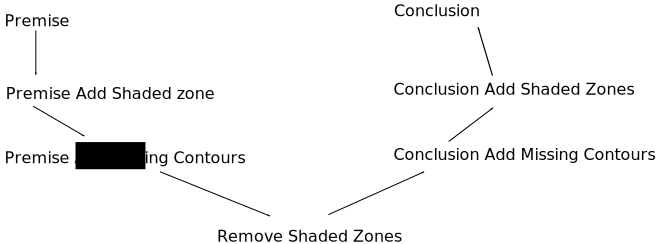
\includegraphics[scale=0.7]{images/unitary.png}
\caption{The order for writing the proof}
\label{unitary}
\end{figure}

\subsubsection{Proof Example}

To make the algorithm easier to understand an example is provided below that shows how the algorithm should be applied to reach the desired result. Figure \ref{d12} is the premise diagram and figure \ref{d11} is the conclusion diagram.

\begin{figure}[h]
\begin{minipage}[h]{0.5\linewidth}
\centering
\includegraphics[scale=0.5]{images/d11.png}
\caption{Premise Diagram}
\label{d11}
\end{minipage}
\hspace{0.5cm}
\begin{minipage}[h]{0.5\linewidth}
\centering
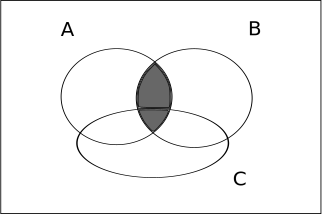
\includegraphics[scale=0.5]{images/d12.png}
\caption{Conclusion Diagram}
\label{d12}
\end{minipage}
\end{figure}

Starting with the premise, the first step as stated above is adding the missing zones and clearly the zone $ (AB , ) $ is missing and needs to be added to the diagram. The resulting diagram is figure \ref{d11-1}. Second step is checking for missing contours that exist in the conclusion diagram but not in the premise diagram. Obviously contour $ C $ is missing and has to be added to the diagram. The resulting diagram is figure \ref{d11-2}. Considering the abstract syntax of the diagram, notice that by adding the new contour, new zones are also created which have to be added to the diagram. Now the zones that exist in this diagram are $ \lbrace (A, BC), (B, AC), (C, AB), (AB, C), (BC, A), (CA, B), (ABC, ), ( , ABC)  \rbrace $.\\
 
Considering the conclusion diagram it is clear that zones $ \lbrace (AB, C), (ABC, ) \rbrace $ are missing and need to be added to the diagram using the add shaded zone rule. Adding the missing zones to the diagram results in the diagram provided in figure \ref{d12-1}. The second step is to add the missing contours to the diagram, but clearly there is no missing contour. Therefore no action is required at this stage. Now the zones that exist in this diagram are $ \lbrace (A, BC), (B, AC), (C, AB), (AB, C), (BC, A), (CA, B), (ABC, ), ( , ABC)  \rbrace $.\\ \\

Both diagrams ( $ d^L_{1} $  and $ d^Z_{2} $) are in their normal form and can be compared now. By looking at the shaded zones in $ d^Z_{2} $ and $ d^L_{1} $, it is obvious that there are no shaded zones in $ d^Z_{2} $ that are not shaded in $ d^L_{1} $. Therefore a proof exists for proving $ d_{2} $ follows from $ d_{1} $. Note that in this special case $ d_{1} $ follows from $ d_{2} $ as well.

\begin{figure}[h]
\centering
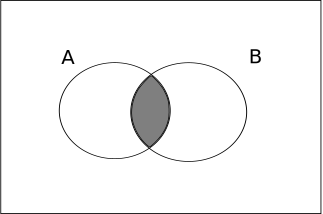
\includegraphics[scale=0.7]{images/d11-1.png}
\caption{$ d^Z_{1} $ - After applying add shaded zone rule}
\label{d11-1}
\end{figure}


\begin{figure}[h]
\centering
\includegraphics[scale=0.7]{images/d11-2.png}
\caption{ $ d^L_{1} $ - After adding the missing contour}
\label{d11-2}
\end{figure}


\begin{figure}[h]
\centering
\includegraphics[scale=0.7]{images/d12-1.png}
\caption{ $ d^Z_{2} $ - After adding missing zones}
\label{d12-1}
\end{figure}

The next step is writing the proof. Following the proof writing algorithm, the proof is:

\begin{enumerate}
\item Starting with $ d_{1} $ in figure \ref{d11}.
\item The next diagram is $ d^Z_{1} $ (figure \ref{d11-1}).
\item The next diagram is $ d^L_{1} $ (figure \ref{d11-2}).
\item Removing shaded zones from $ d^L_{1} $ that are not shaded in $ d^Z_{2} $ is not necessary because none exist.
\item Removing contour labels from $ d^L_{1} $ that are not in $ d^Z_{2} $ is not necessary because none exists.
\item Removing zones from $ d^L_{1} $ that are not in $ d_{2} $ is necessary because the zones $ (AB, C) $ and $ (ABC, ) $ do not exist in $ d_{2} $. The resulting diagram is $ d_{2} $. 
\end{enumerate}

Accoridng to the proof written above, by starting from $ d_{1} $ it is possible to reach $ d_{2} $ after applying each step to the diagrams.


\newpage
\section{Project Design}
\label{sec:design}

In this section the process of designing this project is discussed in detail. Also the findings from the extensive research that was carried out on software design, is provided in a number of arguments that elaborate on software design.
 
\subsection{Initial Steps}
Usually it is expected to start a project by investigating the problem, reviewing available resources and designing a domain model to illustrate the problem and understanding the requirements completely. However this is not how this project started which was a very troublesome mistake. This mistake caused the design of the project to be changed every week and rewriting the code and changing the way different classes interacted with each other. Rushing into implementation can possibly be the most time consuming mistake that was made during the process of this project. This one mistake led to producing a very inaccurate plan which mostly did not work out the way it was expected. Most of these problems were because of lack of knowledge in the area of design and problem solving techniques. However after understating how each step should have been done, the new techniques were adopted and the strategy of proceeding towards completing the project changed in the course of implementation.

\subsection{Design Methodology and Prioritization}
Design methodologies or "software development processes" are different ways that software developers can follow to produce their product. There are a number of design methods that can be used for each project and depending on the specific characteristics of each method and sometimes personal preference one method can be chosen and used. The popular design methods are extreme programming, agile software development, unified process (UP), waterfall method and SCRUM \cite{Agile_book}.\\
Also the term design patterns needs to be defined before moving on to discussing the design process of this project. Christopher Alexander says, "Each pattern describes a problem which occurs over and over again in our environment, and then describes the core of the solution to that problem, in such a way that you can use this solution a million times over, without ever doing it the same way twice" \cite{Gof_book}. 

Extreme Programming or XP for short is a design method that is lightweight, efficient, low-risk, flexible, predictable and scientific way to develop software \cite{Kent_book}. It is distinguished from other methodologies by
\begin{itemize}
\item Its early, concrete, and continuing feedback from short cycles.
\item Its incremental planning approach, which quickly comes up with an overall plan that is expected to evolve through the life of the project.
\item Its ability to flexibly schedule the implementation of functionality, responding to changing business needs.
\item "Its reliance on automated tests written by programmers and customers to monitor the progress of development, to allow the system to evolve, and to catch defects early".
\item "Its reliance on oral communication, tests, and source code to communicate system structure and intent".
\item "Its reliance on an evolutionary design process that lasts as long as the system lasts".
\item "Its reliance on the close collaboration of programmers with ordinary skills".
\item "Its reliance on practices that work with both the short-term instincts of programmers and the long-term interests of the project".
\end{itemize}
XP is designed to work with projects that can be built by teams of two to ten programmers, that are not sharply constrained by the existing computing environment, and where a reasonable job of executing tests can be done in a fraction of a day. For more detail refer to \cite{Kent_book}.\\

Agile development methods apply timeboxed iterative and evolutionary development, adaptive planning, promote evolutionary delivery, and include other values and practices that encourage agility rapid and flexible response to change. It is not possible to exactly define agile methods, as specific practices vary. However, short timeboxed iterations with adaptive, evolutionary refinement of plans and goals is a basic practice various methods share \cite{Agile_book}. The agile principles are 
\begin{itemize}
\item "Highest priority is to satisfy the customer through early and continuous delivery of valuable software."
\item "Welcome changing requirements, even late in development. Agile processes harness change for the customer's competitive advantage".
\item "Deliver working software frequently, from a couple of weeks to a couple of months, with a preference to the shorter time scale".
\item "Business people and developers must work together daily throughout the project".
\item "Build projects around motivated individuals. Give them the environment and support they need, and trust them to get the job done".
\item "The most efficient and effective method of conveying information to and within a development team is face-to-face conversation".
\item "Agile processes promote sustainable development".
\item "The sponsors, developers, and users should be able to maintain a constant pace indefinitely".
\item "Continuous attention to technical excellence and good design enhances agility".
\item "The best architectures, requirements, and designs emerge from self-organizing teams".
\item "At regular intervals, the team reflects on how to become more effective, then tunes and adjusts its behaviour accordingly".
\end{itemize}
For more details refer to \cite{Agile_book}.\\\\

SCRUM is another design method that appears simple, yet has practices that deeply influence the work experience and that capture key adaptive and agile qualities. Scrum's distinctive emphasis among the methods is its strong promotion of self-directed teams, daily team measurement, and avoidance of prescriptive process. Some key practices include \cite{Agile_book}: 

\begin{itemize}
\item Self-directed and self-organizing team
\item No external addition of work to an iteration, once chosen
\item Daily stand-up meeting with special questions
\item Usually 30-calendar day iterations
\item Demo to external stakeholders at end of each iteration
\end{itemize}

\subsection{Prioritization Of Non-Functional Aspects}
\label{guideline}

In this project a specific design method was not chosen because these design methods are more concerned about customers and development team and they do not discuss issues that an individual project has to deal with. But this does not mean that they cannot be used with individual projects, they can be modified and used with individual projects as well. However there are a number of issues which are not mentioned with these methods. 

\begin{itemize}
\item How one starts the process of designing?
\item How can the designer make decisions in order to create an acceptable design?
\item In what circumstances does the designer need to use design patterns?
\end{itemize}

Of course the assumption is that the designer already knows about these issues from previous experience. But for an amateur designer who does not have the necessary experience it is a difficult and time consuming process to make decisions on how to design a piece of software and how to incorporate the different design aspects such as extensibility, reuse, etc in the project. However it seems that there is a simple solution to this problem which is prioritization of non-functional aspects of the design. This means if the designer has a guideline on the importance of different design aspects for having a good design he can easily make decisions on how to proceed in different stages of the design. Some of the non-functional aspects of the design which need to be prioritized are  

\begin{enumerate}
\item Extensibility : How extensible should the system be?
\item Reusability : Is this code going to be reused in the future?
\item Modularity : How modular should the system be?
\item Size : Is the number of lines of code important?
\item Simplicity : How simple should the design be? also who is going to use this design?
\item Maintainability : How important is the maintainability?
\end{enumerate}
In none of the popular software development processes these points are discussed apparently because the designer is supposed to know these before starting to design. However by extending these development processes and incorporating the prioritization of non-functional aspects of designing it simplifies the process of decision making during different stages of the design for both amateur and experienced designers. This prioritization provides the guidelines necessary for whether to use a design pattern and how the programmer should write the code.\\
At the start of this project because of lack of understanding of design no guideline was set before starting the design and this caused the design to change frequently. The main reason for that was the most important desired outcome for the design was unknown, the whole point was to have a nearly perfect design which contained all the above points and was fully compatible with all object oriented design principles. Such a vague, unclear and inaccurate goal caused the design to change because of gaining more knowledge about design in general and also the tendency towards using design patterns as it was thought the more design patterns you use the better your design is. After understanding these points and discovering that prioritization of different non-functional aspects of the design and clearly identifying the most important outcome of the design can change the way a designer makes decisions, the entire process became much simpler and it was possible to create the design which was much more stable compare to the other designs which changed fundamentally every week. \\
After learning more about design this guideline was produced for this project which helped significantly to create the more stable design. The guideline for this project is the below list.
\begin{enumerate}
\item The most important outcome in this project is to complete the automated prover for both unitary and compound diagrams. Therefore the size of the program matters because writing more code requires more time which in this project time is very limited. So the first important priority is less coding (smaller size).
\item It is very important to have this code maintainable as it might be used later by other programmers.
\item Modularity. It is important because some of the modules can be used for other purposes as well because some of them can be helpful in solving other problems i.e. the binary tree creation module.
\item Extensibility is useful because this code "might" be used in the future to be extended in order to create a more accurate and efficient prover. It is important not to confuse extensibility with maintainability. Extensibility means to extend the program by adding new features to it but maintainability means that if there is a bug or if a task that the program is performing needs to be changed, fixing or changing it is not difficult and can be done by other programmers as well. Maintainability does not usually mean introducing new features to the software.
\item Reusability is important if the code is going to be used later on but is not absolutely necessary. This does not mean reusability is not important in implementation, it only means it is not absolutely important to make the design reusable so it can be applied to other problems.
\item Simplicity is important to keep the design simple and understandable however it is not strictly necessary because the users of the system are mathematicians and programmers who do not have difficulty understanding the aspects of the design and the code.
\end{enumerate}

The importance of this prioritization is more conceivable when an amateur designer wants to decide whether or when to use a design pattern. In the gang of four book \cite{Gof_book} the benefits of each pattern is given clearly and by reading each benefit if the pattern is relevant to what is needed in the design, the designer might think that using the pattern is a good idea whether it is necessary or not. As the pattern provides such promising benefits. Therefore the designer decides to use the pattern. However if the designer had a guideline on what is most important in the design, the process of making decision would be based on what is necessary rather than what is beneficial. This will protect the designer from unnecessary change to the design and therefore the implementation of the software. For instance in this project there is an algorithm for creating binary trees for constructing a compound diagram. Designing and implementing this algorithm can use a number of different patterns which are very beneficial and there are good reasons why to use them. These patterns include visitor pattern, template method pattern, strategy pattern and composite pattern. Each one of these patterns provide a set of very promising benefits, for example a template method pattern defines the skeleton of an algorithm in an operation, deferring some steps to subclasses. Template Method lets subclasses redefine certain steps of an algorithm without changing the algorithm's structure \cite{Gof_book}. It is possible to say that it might be necessary to create the binary tree in a different way as the project is extended. So it is a good idea to use the template method pattern here. But as stated above in the guideline for this project the most important outcome is less coding and completing the program in the short time that is provided for implementation and also extensibility is priority number 4. Therefore it is not necessary to use this pattern even though it is beneficial.\\

Moreover, prioritization of non-functional aspects of design can solve another problem in designing which is defining what is meant by the relative terms such as "good design" or "better design" or "bad design". Because the set of guidelines (or list of priorities) that is created provides the ability to be able to compare and contrast different designs by checking which design satisfies more of the priorities in the correct order. Therefore the design that satisfies more of the priorities can be considered as the "better design" and this reduces the ambiguity of the term "better". 

\subsection{Design Patterns}
\label{Design_Patterns}
Experienced software engineers have built a repository of both general principles and idiomatic solutions that guide the process of creation of software. Design patterns help different software engineers from different backgrounds to be able to communicate with each other in more effective way because the software engineers who understand patterns and the design terminology can discuss and explain different problems in a more general way that everyone else also understands. More accurately, a pattern is a named description of a problem and solution that can be applied to new contexts, it provides guidance on how the problem should be solved in a way that it obeys the important design principles \cite{Larman_book}. 

\begin{quotation}
The GRASP patterns are a learning aid to help one understand essential object design, and apply design reasoning in a methodical, rational, explainable way. This approach to understanding and using design principles is based on patterns of assigning responsibilities.
\end{quotation}

The patterns that are used in this project are 
\begin{itemize}
\item Factory Method: This pattern defines an interface for instantiating objects. This pattern lets the decision of which class to instantiate to the class's subclasses.
\item Singleton: Ensures that a class only has one instance and provides global access to it \cite{Gof_book}. 
\item Façade: Provides a general interface to a set of interfaces in a subsystem. This higher level interface makes the subsystem easier to use.
\item Builder: Separate the construction of a complex object from its representation so that the same construction process can create different representations \cite{Gof_book}.

\end{itemize}

\subsection{General Responsibility Assignment Software Patterns}
\label{Grasp}
One of the significant aspects of objected oriented design is understanding GRASP (General Responsibility Assignment Software Patterns) which helps remarkably in the process of designing. GRASP explains fundamental principles of object design and responsibility assignment expressed as patterns. According to \cite{Larman_book}
\subsection{Prioritazation Of Non-Functional Aspects}
In this project a specific desig
\begin{itemize}
\item Information Expert: Assigning responsibilities should be left for information expert, the class that has the necessary information to fulfil the responsibility. 
\item Creator: If any of the following cases is true then there should be a class "ObjectCreator" that creates objects of class "ClassA".
\begin{itemize}
\item "ObjectCreator" aggregates "ClassA" objects.
\item "ObjectCreator" contains "ClassA" objects.
\item "ObjectCreator" records instances of "ClassA" objects.
\item "ObjectCreator" closely uses "ClassA" objects.
\item "ObjectCreator" has the initializing data that will be passed to "ClassA" when it is created (thus "ObjectCreator" is an Expert with respect to creating "ClassA").
\end{itemize}  
\item Low Coupling: Assign a responsibility so that coupling remains low. Coupling is a measure of how strongly one element is connected to, has knowledge of, or relies on other elements \cite{Larman_book}. Classes with strong coupling rely on many other classes, changing one of the classes that the strongly coupled class rely on will also need local changes to the strongly coupled class. Therefore it is not desirable to have strong coupling in the design as much as possible.
\item High Cohesion: Cohesion (or more specifically, functional cohesion) is a measure of how strongly related and focused are the responsibilities of an element \cite{Larman_book}. An element with highly related responsibilities, and not a great deal of work to do, has high cohesion. A class that has numerous responsibilities and performs many unrelated tasks is undesirable because of (for more detail refer to \cite{Larman_book}):
\begin{itemize}
\item It is hard to understand.
\item It is hard to reuse.
\item It is hard to maintain.
\item Is constantly affected by change.
\end{itemize}

\item Controller: A controller is an internal part of the system that does not have a user interface and is responsible for dealing with system events. This pattern is provided to handle system events. For instance when a button is pressed in an application the event should be sent to the button controller to decided what the next step is.
\item Polymorphism: This pattern deals with situations where behaviours vary based on the type of an object. Assigning responsibilities for the particular behaviour using polymorphic methods (or operations) makes the program easily changable and extensible because it is logical to use polymorphism rather than using conditional if-else statements to vary operations based on types. The word "polymorphism" means giving the same name to methods in different objects. 
\item Fabrication: In situations where assigning responsibilities might violate low coupling, high cohesion, reuse or other important principles of design, it is essential to assign a highly cohesive set of responsibilities to an artificial class that does not represent a problem domain concept and is just a new concept created to support high cohesion, low coupling, and reuse. This class that is the product of imagination is called fabrication. 
\item Indirection: This pattern is provided to solve the problem of coupling between objects. It suggests that responsibilities should be assigned to an intermediate object to mediate between other components or services rather than directly coupling components or services.
\item Protected Variations: This pattern protects different elements from the variations on other elements of the system. By assigning responsibilities to create a stable interface around them (interface in this case is interpreted in the most general sense, it does not have the same meaning as Java's interface).  
\end{itemize} 

Considering these factors it seems GRASP covers a great deal of important aspects of a "good" design. Applying these patterns to the design of this project helped tremendously in reduction of lines of code and also increased the speed of implementation. When the design is understandable and follows the important principles of design, there is a relativity high probability that the number of bugs will not be as large as it would be with a design which does not follow the principles. Certainly this was the case in this project, after the "better" design was implemented, debugging became easier and some previous bugs disappeared. 

\subsection{Domain Model}
The domain model is the general model or the conceptual model that describes the various entities involved in the system and the interactions between each entity in that system. At the start of the design process this model was not produced as it was assumed that the problem was clearly understood. Not producing this model caused the design to be changed again. The model that is produced for this system is provided in figure \ref{model}. As the model shows the prover uses diagrams and applies various reasoning rules to them and then if there is a proof it will perform the necessary operations (which is writing the proof). This is the modelling of the domain at the very basic level.

\begin{figure}[h]
\centering
\includegraphics[scale=0.7]{images/domainModel.jpeg}
\caption{Domain Model}
\label{model}
\end{figure}


\subsection{Process of Designing}
At the start it was decided not to design the entire project up front because it will undoubtedly be inaccurate and change when the process continues. Each week there were a few set tasks set by the supervisors to complete for the following week. The first task was implementing the "add contour" rule. The tasks for the first few weeks of the project were implementation of
\begin{itemize}
\item Remove Contour
\item Remove shaded zone
\item Add shaded zone
\item File structure to capture the abstract syntax of a unitary diagram.
\end{itemize}

The designs that was produced in the second and third weeks of the project did not comply with object oriented principles because of lack of understanding of object oriented design and also assuming that contours and zones are primitive data types rather than objects. This mistake of having zones and contours as primitive data type increased the size of the program unnecessarily because every time for checking whether or not a zone or a contour is equal to another zone or contour, it was required to write the equality check but if they were objects the equality check could have been set as each object's method and could have been used by just calling the method. Figure \ref{2nd} and \ref{3rd} and \ref{4th} show the designs produced in the second, third and fourth weeks of the project. Obviously the first month of the project the progress was not as good as it could have been and the only reason that the progress was not acceptable was mainly because of lack of understanding of design which it was mentioned repeatedly earlier.  Another reason for frequent change in the design was that when a designer does not know why the design that he has produced is the way it is, if he finds a different way that seems to be better he has no option but to change the design. This was the case for this project in the first two to three months of the project.

\begin{figure}[h]
\centering
\includegraphics[scale=0.7]{images/2nd.jpeg}
\caption{Class Diagram in second week}
\label{2nd}
\end{figure}

\begin{figure}[h]
\centering
\includegraphics[scale=0.7]{images/3rd.jpeg}
\caption{Class Diagram in third week}
\label{3rd}
\end{figure}

\begin{figure}[h]
\centering
\includegraphics[scale=0.5]{images/4th.jpeg}
\caption{Class Diagram after the fourth week}
\label{4th}
\end{figure} 

After about 6 weeks the project reached to the point where it was ready to check to see whether a proof exists for two given diagrams. The diagram shown in figure \ref{5th} was the result of the 6 weeks of working on the project. This design provides the necessary functionality that is needed for the system but it is not necessarily extensible for the later stages such as  incorporating compound diagrams. After about 8 weeks the project was able to check and write a proof given two unitary diagrams. Although later it was discovered that the project had a few bugs which caused the proof process to be incorrect. This bug was discovered after performing a number of tests manually. There were a number of advantages with this design which are

\begin{itemize}
\item It is relatively a loosely coupled system. Every class has its own responsibilities and not all classes are dependent solely on the other classes.
\item Contour and zone classes are added and now they can be treated as objects rather than primitive types.
\item Overall less code is needed compare to the previous designs.
\end{itemize}

\begin{figure}[h]
\centering
\includegraphics[scale=0.5]{images/5th.jpeg}
\caption{Class Diagram After 6 weeks}
\label{5th}
\end{figure}

The experience that was gained during designing the first part of the program (unitary diagram proofs) created a compelling reason to learn more about design and object oriented programming before starting the second part of the design for compound diagrams as there are a lot of patterns and principles that are useful for designing such a system. This conviction was a compelling reason to learn as much about design as possible in the time available before starting the second stage of the project. Understanding objected oriented design principles and also all the 23 patterns included in \cite{Gof_book} made the process even more tricky because understanding more requires more thinking about the design and also considering all the other available options which are possible. Furthermore the uncertainty that was created because of not knowing which way is the correct way to proceed with the design consumed a great deal of time. Until the point about the importance of prioritization of the non-functional aspects of design was discovered which made decision making about what is the best path to go much easier.\\

As far as it was understood during the research process designing does not have a scientific approach developed for it yet and it is essential to have useful experience before starting to design. Unfortunately this practical experience that "experienced" designers have is not documented anywhere and therefore it is necessary at times to adopt personal methods that seem to be logical in designing. Even though the personal methods might not be as effective as expected. On the whole, the time that was spent on researching on designing was very effective and opened a new chapter in understanding how designing should really be. With this understanding the design that is introduced in section \ref{class_diagram} was the latest class diagram that was designed for this project.    

\subsection{Class Diagram Explanation}
\label{class_diagram}
The final class diagram that was produced is represented in figure \ref{des10} (all methods and attributes are removed to fit the diagram in one page, the sourcecode of the program is provided in the CD-ROM provided). This diagram will probably be changed slightly for implementing the compound diagrams proof algorithm but currently it seems to be an acceptable choice. The features in this design are listed below to indicate what advantages this design has.

\begin{itemize}
\item Each class has one major responsibility.
\item The system is relatively loosely coupled.
\item Indirection is one of the important aspects in design which is obeyed in this design \cite{Larman_book}. Different classes are provided whenever possible to mediate between objects rather than directly coupling the objects. For instance class "TED" mediates between different components of the system such as "Prover" and "DiagramLoader".
\item Creator pattern is used in the design whenever necessary. For example the creation of a compound diagram is not done in "TED" but it is done in "CompoundCreator" class. 
\item Interfaces are provided so clients are not exposed to the inner parts of the system. They just interact with the interface.
\item A few necessary and useful patterns are used.
\item Cohesion in the design is considered carefully and it is achieved to a certain extend. All classes have focused, manageable and understandable responsibilities which allow objects to interact with each other easily.
\item Fabrication is also used in this design whenever necessary. For instance the class "DiagramLoader" is provided to achieve low coupling and cohesion.
\item Controller pattern is also used in this design to deal with different commands that the user inputs into the program.
\item Information expert pattern is used to guide how the assignment of responsibilities should be done.
\end{itemize}

\begin{figure}[]
\centering
\includegraphics[angle=90, scale=0.4]{images/des10.jpeg}
\caption{Final Class Diagram}
\label{des10}
\end{figure}

\newpage
\subsection{Classes Explanation}

\subsubsection{Class: TED (Theorem prover for Eulre Diagrams)}
This class is responsible for handling interactions between the user and the system. It mediates between the user and different parts of the system. For example if the user enters the command to load a diagram "TED" handles the command by sending a message to "DiagramLoader" class to load the diagram. In the testing section \ref{sec:Testing} screen-shots are provided to show how the program works.

\subsubsection{Class: DiagramLoader}
A diagram is stored in a file (which can be a text file), using the diagram's abstract syntax. This file has a specific style which needs to be followed exactly. In order to be able to load the diagram it is necessary to

\begin{enumerate}
\item Read the file.
\item Tokenize the file.
\item Prepare the attributes for diagram object.
\item Check the syntax.
\item Create the diagram object.
\end{enumerate}

All these operations are necessary to be done in order to be able to create a diagram object. Of course all of them could have been done in one class, however, following object oriented design principles each one of these operation should be assigned to specific classes that can fulfil the necessary requirements. As the result of applying these principles the following classes are essential to be created (which are explained in the next sections).

\begin{itemize}
\item DiagramCreator
\item LexicalAnalyser
\item SyntaxChecker
\item Parser
\end{itemize}

Having designed loading a diagram into memory in this way has the advantages of 
\begin{itemize}
\item Low coupling
\item Correct assignment of responsibilities.
\item Altering one of the classes would not affect the other parts.
\item GRASP patterns are used.
\item The diagram loading component is independent of other parts of the system which means that it can be reused.
\end{itemize}

After all of the necessary prerequisite stages are completed DiagramLoader returns a diagram to the caller. It is important to notice DiagramLoader can also be seen as a Facade pattern becuase it hides a number of classes from it's client and handles the details by itself and returns the desired output to the client.

\subsubsection{Class: LexicalAnalyser}
LexicalAnalizer in this system is responsible for tokenizing the diagram file. It is very similar to a compiler lexical analyser but it does not do the same amount of work.

\subsubsection{Class: Parser}
This class is responsible for sorting the tokens into different sets which are needed to complete different attributes of a diagram object.

\subsubsection{Class: SyntaxChecker}
This class is responsible to check to see whether the abstract syntax of the diagram is correct or not. If it is not, it will take the necessary actions to inform the user.

\subsubsection{Class: DiagramCreator}
DiagramCreator as it's name suggests is responsible for creating the diagram object. It receives the required attributes and then creates the object.

\subsubsection{Class: ProofWriter}
This class is primarily responsible to save the generated proof to a file called "proof.txt". It is called from TED class.

\subsubsection{Class: Prover}
Prover class is an abstract class that its methods are implemented by UnitaryProver and CompoundProver. It is provided to be an interface so the clients can use the interface and not be exposed to the internal parts of the system.

\subsubsection{Class: UnitaryProver}
This class implements certain methods of the Prover class and it is only responsible for unitary diagram proving algorithm.  

\subsubsection{Class: CompoundProver}
CompoundProver is provided to apply the compound diagram proving algorithm. It is responsible only for proving compound diagrams and it does not have any knowledge of any other aspects of the program. 

\subsubsection{Class: UnitaryProverCreator}
This class is part of a factory method pattern that is introduced in this design. The factory method is used to allow subclasses (UnitaryProverCreator and CompoundProverCreator) decide which prover object should be instantiated. This class implements the factory method (implementation is discussed in section \ref{sec:Implementation} for creating an object of UnitaryProver.

\subsubsection{Class: CompoundProverCreator}
Similar to the previous class, this class is also a part of the factory method pattern that is introduced in this design. This class is responsible for instantiating an object of the class CompoundProver.

\subsubsection{Class: ProverCreator}
ProverCreator declares the factory method, which returns an object of type Prover. Clients will use this class whenever a prover object is needed and this allows it's subclasses to determine which type of prover object they should create (UnitaryProver or CompoundProver). The reason for using a factory method is that it is unknown at runtime which type of a prover should be used until the user inputs the command for proving. Also factory method provides flexibility in this design because it allows subclasses to redefine the way objects of different types (i.e. CompoundProver) are created by just changing the particular subclass of ProverCreator. 

\subsubsection{Class: Rules}
This class is the superclass of classes UnitaryRule and CompoundRule. As all CompoundRules and UnitaryRules are still rules this class is provided to incorporate this relationship.
 
\subsubsection{Class: UnitaryRule}
This class has all rules that can be applied to unitary diagrams. It is a subclass of Rules class.

\subsubsection{Class: CompoundRule}
CompoundRule has all rules that can be applied to compound diagrams. It's primary responsibility is to let the clients apply different rules.

\subsubsection{Class: Traversal}
Compound diagrams are represented as binary trees in this system to capture their structure. It is required to be able to traverse through the binary tree in order to read the tree structure and perform the necessary operations. This class is provided as an interface which declares a number of methods that are essential for tree traversal. This interface is provided because at this stage of the project in-order tree traversal is the only type of traversal needed, however, it might be necessary in the future to implement pre-order or post-order tree traversals as well. So by providing this interface the system can be more extensible and allow extensions to be applied in a more structured way (i.e. implementing the interface for a pre/post-order traversal).\\

%In this part of the system (the tree traversal component) visitor pattern and strategy pattern could have been used for the following reasons:
%\begin{itemize}
%\item 
%\end{itemize}

\subsubsection{Class: InorderTreeTraversal}
This class's primary responsibility is to traversing the given binary tree in an in-order fashion. In-order tree traversal is described in section \ref{inorder}.

\subsubsection{Class: Diagram}
Diagram class is the superclass of UnitaryDiagram and CompoundDiagram. Because both unitary diagrams and compound diagrams are still diagrams, it is acceptable to provide a class (Diagram Class) that represents this relationship correctly. Therefore this class is provided to depict this relationship between these diagrams and also if in the future a different type of diagram needs to be introduced to the system, by extending this class it can be treated as other diagrams.
 
\subsubsection{Class: UnitaryDiagram}
UnitaryDiagram class is the abstraction of a unitary diagram. It captures all attributes of a diagram's from it's abstract syntax and provides a diagram. This class does not perform any processing on the diagram at all, it is only assigned the responsibility of representing a diagram.

\subsubsection{Class: Contour}
Contour class as it's  name suggests, is the abstraction of a contour. In the first designs contour was not an object but rather a primitive data type (string). According to \cite{Larman_book} anything that can be made into an object, should be made into an object. Also as explained in the previous sections contours are sometimes need to be compared to each other or need some action to be performed on them. Clearly these are very compelling reasons to introduce contours (and zones) as a separate object and doing this did pay off during implementation phase as less coding was necessary because Contour class had all the necessary operations encapsulated in itself which could be used whenever required.
  
\subsubsection{Class: Zone}
Similar to the Contour class, this class is an abstraction of zone. Zones also were not described as objects originally and they were defined using primitive data type, string. As explained in the previous section, not describing zones as objects is not an intelligent way of designing. Therefore for the same reasons as before this class was introduced and it's responsibility was set to represent zones.

\subsubsection{Class: CompoundDiagram}
This class is responsible for holding the compound diagram's binary tree which is created and passed to it. It has the operations essential for a compound diagram and also it has operations to display what the compound diagram is. But it does not have the responsibility of performing any modifications to the diagram by itself. \\
It is important to note that, in this case it is possible to use the composite pattern to represent a compound diagram, however, according to the priotrization of non-functional aspects of the design, it was not a crucial necessity to use the pattern, it was possible to create the tree like structure without using the pattern and also keep the design relatively simple.

\subsubsection{Class: CompoundCreator}
As the name says, this class is responsible for creating the CompoundDiagram object. It uses a number of other classes to construct the binary tree of the compound diagram. 

\subsubsection{Class: CompoundTree}
CompoundTree is the abstraction of a binary tree. It is important to note that these binary trees might not always be a proper binary tree (a tree that all nodes apart from the leaves have two children) because of the "not" ($ \neg $) operator only has one child. In fact this class is created to incorporate the idea of a binary tree as an object. A Binary tree is a set of linked nodes and it does not need to be contained in another object such as a tree, but it is easier to understand where there is a class that represents the abstraction of a tree which can hold the set of nodes. That is the reason why this class is created, to make the design more understandable.

\subsubsection{Class: CompoundNode}
CompoundNode is a representation of a node. This class is provided to play the role of a node in a tree. It has the necessary attributes that allows a node object to be linked to other node objects. It does not modify or perform any operation on the node in any way.

\subsubsection{Class: DiagramHolder}
This class is responsible for storing diagrams and providing a number of operation that can be applied to that set of diagrams. DiagramHolders are used where it is required to hold a set of diagrams in a collection e.g. it is necessary to store diagrams after each operation in the process of prvoing them. Creating this class redueces the size of the program because the operations that are necessary to be done on a collection of diagrams does not have to be re-written each time they are needed.

\subsubsection{Class: SetMaker}
This class is responsible for checking if a C++ standard library Vector's elements are all unique and if they are not it will make them all unique (by removing the duplicate elements). In section \ref{vectors} the reason why C++ STL sets where not used instead of vectors. 

\subsubsection{Class: TreeBuilder}
Building a tree (CompoundTree object) is the responsibility of this class. TreeBuilder uses an ExpressionTokenizer and an InfixToPostfix object to prepare the required raw data before creating the tree. This class is inspired from the idea of the Builder pattern which is used to seperate the construction of a complex object from it's representation so the same construction process can be used to create different representations. By seperating the construction of a tree, it is possible to change the process of constructing a tree without changing any other classes, if it was necessary.

\subsubsection{Class: ExpressionTokenizer}
As the user needs to input the compound diagram to the system using an expression that describes the compound diagram, it will be required to tokenize the expression. Because of this reason this class is provided to fulfil that responsibility.

\subsubsection{Class: InfixToPostfix}
For processing an expression that is going to be made into a tree, it is required to know which node is the root node. Finding a root node is not a very straight forward job because it needs to deal with a lot of checkings but there is a very straight forward way of finding the root node and it's left and right children. By converting the expression into an infix expression it becomes so easy to spot the root node, it is the last node in the infix expression. For example the statement 
$$ (d_{1} \wedge d_{2}) \vee ( \neg (d_{3} \vee d_{4}))  $$
will be converted to an infix expression 
$$ d_{1} d_{2} \wedge d_{3} d_{4} \vee \neg \vee $$
which does not use any brackets and it takes no effort to spot the root node.
\newpage
\section{Implementation}
\label{sec:Implementation}
This section is provided to explain the important aspects of implementation in this project. It includes all the key information about the implementation of this project which is useful to be noted. The project's code is on the CD-ROM provided and can be read if necessary.
 
\subsection{Language}
The choice of a language was not a major issue in this project because any objected oriented language could have been used for this project. It was possible to choose Java as the programming language because of 

\begin{enumerate}
\item Having past experience with the language.
\item Low possibility of having language related problems.
\item Not needing to manually perform memory management.
\item Java programs are multi-platform which means they do not need to be recompiled for running on Windows or Linux.
\end{enumerate}

The advantages that Java has makes it a suitable language for this project, but this project is an experimental project which means that one of it's most important criteria is learning. Also because of personal interest in learning new languages, it was decided to use C++ as the programming language of this project. Although C++ might not seem to be the best programming language for this project but it has some nice features that are quite useful which are listed below:

\begin{enumerate}
\item Pointers: A pointer is a variable that holds a memory address. This address is the location of another object (typically another variable) in memory. For example, if one variable
contains the address of another variable, the first variable is said to point to the second \cite{C++Ref_book}.
\item Efficiency: Programs written in C++ are normally more efficient compare to other languages. Comparing to Java, C++ programs are remarkably faster because there is no virtual machine in C++.
\item Templates: The template is one of C++'s most sophisticated and high-powered features. In a generic function or class, the type of data upon which the function or class operates is specified as a parameter. Thus, it is possible to use one function or class with several different types of data without having to explicitly recode specific versions for each data type \cite{C++Ref_book}.
\end{enumerate}

The disadvantages of C++ which did affect this project were:
\begin{enumerate}
\item Memory Management: Because there is no garbage collection in C++, memory management has to be done manually. For this project not a great deal of memory management was necessary because pointers were not used very often in the first section of the project. But in the second part were pointers were used, some peculiar errors happened which wasted at least a couple of weeks of the implementation time of the project in total.
\item Using C++ standard library is not very user friendly as Java's API or QT's API is. It is possible to use Boost or QT libraries but they both have a learning curve which also requires more time.
\item Errors in C++ are not as nice as they could be. It is difficult at times to spot the place where the error is coming from. In contrast, errors in Java are more clear and it is much simpler to spot where the error is coming from. 
\end{enumerate}

Currently non-hardware related programming can be often done in any of the popular object oriented languages available. So it is more of a personal preference the language that is chosen for a project rather than having compelling facts about why to choose a specific language. Therefore because of personal interest and lack of experience in C++, it seemed to be a valuable learning experience for this project to choose C++ as the programming language, as learning is a very important criterion.\\

\subsection{The Editor}

The editor that was used for this project was Emacs and it was treated as the primary IDE (integrated development environment) for the implementation of this project. Choosing Emacs has its pros and cons, it is an extremely useful text editor but it lacks some of the functionalities that an IDE like Eclipse has. The advantages of Emacs are 

\begin{itemize}
\item The ability of using keyboard for almost everything and not using mice. This functionality speeds up programming quite significantly.
\item Ability to access the command line using Emacs and not needing to switch between the command line and the IDE.
\item Moving the cursor is very efficient in Emacs if the correct shortcuts are used.
\item Extremely customizable for everything. 
\end{itemize}

and its disadvantages are:

\begin{enumerate}
\item Not being able to treat the whole project as one piece. This means that all classes are separate from each other and it is not possible to refactor code as easily as it can be done in Eclipse.
\item Not having debugging tools like Eclipse has, which means that for debugging, command line has to be used and the programmer has to remember all the commands which is slightly difficult.
\item Having no meta-data about the project and the workspace makes it difficult and time consuming to set-up the development environment to start implementing each time.
\item Compiling the project using Emacs is done by using "Make" (there are other tools as well) which is an automated tool for building C++ code. The "Makefile" has to be maintained manually which is also an error prone task at times when the programmer forgets to add the new class to the "makefile" or the order of compiling classes is incorrect.
\end{enumerate}

The experience that was earned during the implementation of this project suggests, use a proper IDE for large projects and if the project is not going to be very large use Emacs.  


\subsection{Why Vectors?}
\label{vectors}

The collection class that is used in this implementation primarily is STL's(Standard Library) vector class. This collection class is used because:

\begin{itemize}
\item It stores elements in the order that they are added.
\item It is possible to access individual elements by their position index.
\item It is possible to iterating over the elements in any order.
\item It is possible to add and remove elements from its end.
\item It does not need to have an iterator object to iterate over elements unlike the STL's Set collection class. 
\end{itemize}

All the collection objects that are needed for "Diagram" objects are in, reality, mathematical sets which means they do not have duplicate elements in them. So it is a reasonable choice to choose a Set collection class which perfectly matches the requirement. However Set class was not used because of not having all the nice features that Vector class has and as a result of this a class called SetMaker, which is explained in Design section, was created to convert a vector object to a set which means to remove any duplicate elements that might exist in the vector.

\subsection{Combination Algorithm}
The most challenging part of the implementation was design and implementation of an algorithm to generate all possible zones from a given set of contour labels. After some research on finding a well defined combination algorithm no standard algorithm was found. Therefore it was necessary to create an algorithm to create all possible combinations of zones of a diagram. \\
Combination in this case means there is no repetitive contour label in any zone. For example, the zone $ (ABC , D ) $ is the same as $ (BCA, D) $ and does not need to be generated again. The best way to explain this algorithm is by a visual example. Note that this algorithm works for generating zones for three or more contour labels. If there are less than 3 contour labels, the generation process is modified slightly to produce the zones.\\

\begin{figure}[h]
\centering
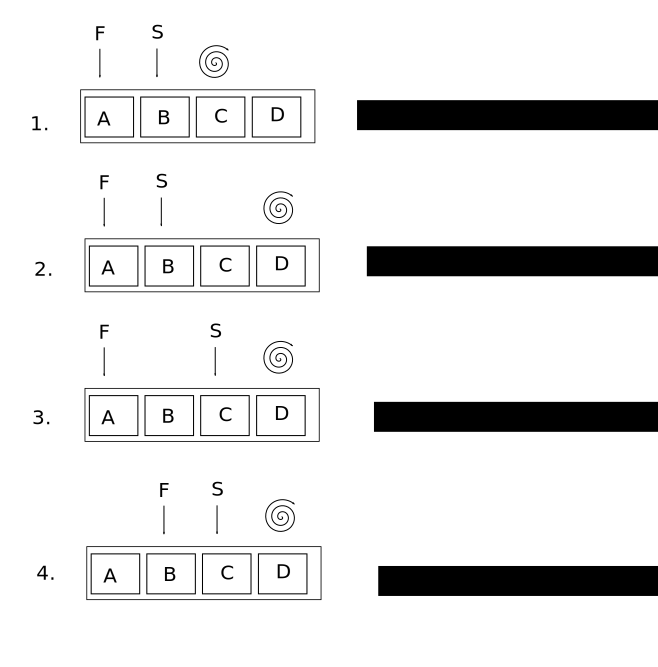
\includegraphics[scale=0.8]{images/combination.png}
\caption{Combination Algorithm Example for Contours {A, B, C, D} }
\label{combination}
\end{figure}

The contour labels in this example are  $ \lbrace  A , B, C, D \rbrace $ and the zones that are going to be generated are:
$$
\begin{tabular}{ r c l }
 	\(\lbrace \)  & \((A, BCD) , (B, CDA) , (C, DBA), (D, BCA), \)\\
   & \((AB, CD), (AC, BD), (AD, BC), (BC, DA), (BD, CA), (CD, BA), \)\\
   & \((ABC, D) , ( ABD, C) , (ACD, B), (BCD, A), \)\\
   & \( (ABCD, ), ( , ABCD)  \)\\
	\(\rbrace \)	
\end{tabular}
$$

The example given in figure \ref{combination} depicts the stage of the algorithm that is creating three-label zones like $ (ABC , C) $. There are a few points that need to be mentioned about how this algorithm works:

\begin{itemize}

\item At each round that the loop runs, the number of characters that are needed increases by 1. For example at the first round the loop just produces one-label zones e.g. $ (A, BCD) $, at the second round it produces two-label zones e.g. $ (AB, CD) $ and so on. 
\item The number of rounds that the main loop runs is the same as the number of available contours.
\item By carefully considering the process of creating zones, it becomes clear that in each round, there are a number of contour labels that are constant for a number of zones. For example in figure (\ref{combination}) zones $ (ABC, D) , ( ABD, C)  $ have $ AB $ in common and their last label changes. The number of constant contour labels is equal to the round number minus one. So at each round, \textit{ round number - 1 } contour labels are needed to be stored and the last contour label has to be retrieved using another loop.
\item First pointer: This pointer which is represented by an "F" in figure (\ref{combination}) holds the index of the starting contour label of the constant part.
\item Second pointer: This second pointer is represented by an "S" in figure (\ref{combination}) holds the index of the last contour label of the constant part.
\item Moving pointer: This pointer is is represented by the curly arrow in figure (\ref{combination}). This pointer iterates through the collection of contour labels to get the last label that is needed for completing the zone.
\item Using first and second pointers makes it possible to create the constant part of the zone and by using the moving pointer the last contour label can be acquired.
\item When the moving pointer reaches the end of the vector of contour labels:
\begin{itemize}
\item If there are more zones left for the current round, the first and second pointers move forward by one. The same process continues.
\item If the second pointer also reaches the end of the vector, move to the next round because there are no more zones left to be generated for the current round.
\end{itemize}

\end{itemize}
By nesting all the essential loops in the main loop that runs for the number of available contour labels, it is possible to generate all the possible zones. However there is a problem with this algorithm which is it's time complexity. The running time of this algorithm is not efficient at all because of the number of loops that will run in each round normally, are nearly 5 which is considered to be a slow algorithm. But it is possible to improve the algorithm by reducing the number of loops and improving the time complexity of the algorithm. According to the prioritization of the non-functional aspects of the system, efficiency is not a requirement for this project and therefore it is not necessary to take any action for making the project more efficient now.


\subsection{Tree Building}
As explained in the design section, in order to be able to construct a compound diagram it is necessary to capture the structure of compound diagrams in a manner that is not ambiguous and also is easy to use. The standard method of dealing with mathematical expressions in computer science is using trees and particularly binary trees for arithmetic expressions. Comparing compound diagram expressions and arithmetic expressions, it is clear that they are relatively similar with one difference. There is no precedence in compound diagram expressions which means that the connectors ($ \vee , \wedge $) and the "not" operator ($ \neg $) do not have priorities over each other, unlike arithmetic expression which have precedence between different operators like $ + , - $  and $ \times , \div $. \\

Before starting the implementation of the tree builder it was assumed that there must exist a well defined, standard and objected oriented method for building binary trees that anyone who needs to have such functionality in their system can simply reuse and adopt the design. After a lengthy research on the methods of designing and constructing a binary tree, no standard method was discovered which means the assumption was wrong. Therefore the tree building module was also designed and implemented according to the guidelines provided in section (\ref{guideline}). The point about the prioritization of non-functional aspects of design was understood while designing and implementing this part of the project because of the numerous ways that were discovered about how to deal with trees. \\

As a matter fact all is needed for constructing a tree is just a node class but in order to make the design more extensible and more understandable it is possible to have another class that represents the whole tree which consists of nodes. The tree class can be used to provide a set of useful functionalities such as 

\begin{itemize}
\item Identifying the root node.
\item Checking the size of the tree.
\item Modifying the entire tree.
\end{itemize}   

\subsubsection{Expression Tokenizing}
In the standard library of C++ there is no class like Java's StringTokenizer available. So it is necessary to have a tokenizer for tokenizing expressions. The way the tokenizer works here is based on the following algorithm

\begin{enumerate}
\item Read the string character by character.
\item Ignore spaces.
\item If a character matches with one of the pre-defined characters:
\begin{itemize}
\item If the character itself has to be a token, tokenize it.
\item If the character has to be in a specific order with some other characters, read ahead until all are matched. Then tokenize it.
\end{itemize} 
\item Add all tokens to a collection.
\end{enumerate}

\subsubsection{Infix to Postfix}
The most important part of building a tree is to identifying the root node and finding the left and right children of all nodes. There are numerous ways that the root node can be identified and then discovering all the other nodes with their children.However in this project one of the most important factors was to implement the code in the most standard way that is both designed and implemented well. Because of this factor and after some research on how to implement a tree, an algorithm was found which inspired the way the infix to postfix algorithm that is used in this project was implemented.\\
The found algorithm is called the Shunting-yard algorithm, this algorithm was created by Edsger W. Dijkstra the renowned computer scientist, to convert mathematical equations specified in infix notation to Reverse Polish notation (RPN) or postfix notation, refer to \cite{edgar_paper} and \cite{shunting_site}. The algorithm is called "shunting yard" because the way it works resembles a rail road shunting yard. The algorithm is explained below in detail.\\
In this algorithm there are 

\begin{itemize}
\item An output queue which stores the operands and operators for the postfix expression that is being created.
\item An operator-stack that is used for keeping operators and brackets while reading the tokens. 
\end{itemize}

According to \cite{shunting_site} the algorithm works as described below:

\begin{itemize}
\item If the current token is an operand, then write it to the output queue.
\item If the token is an operator, then: 
\begin{enumerate}
\item while  token's precedence is less than or equal to precedence of the operator on top of the operator-stack : pop the top operator from the operator-stack and write it to output.
\item Push the token onto the operator-stack.
\end{enumerate}
\item If the token is '(', then push it onto the operator-stack (with precedence - 1).
\item If the token is ')', then:
\begin{enumerate}

\item While the top of the operator-stack is not a '(' : 

\begin{itemize}
\item Pop the top operator from the operator-stack and write it to output.
\item If the operator-stack becomes empty, then a bracket-balancing error has occurred.
\end{itemize}

\item Pop the '(' off the operator-stack; discard it and the token.
\end{enumerate} 

\item Repeat the steps for all tokens that exist.
\item Until the operator-stack is empty: 
\begin{itemize}
\item Pop the top operator from the operator-stack and write it to output.
\item If the top of the operator-stack is a '(' , then a bracket-balancing error has occurred.
\end{itemize}

\end{itemize}
 
To clarify the algorithm an example is provided to make it more understandable. The example in figure (\ref{fig:shunting}) demonstrates how the algorithm performs different operations to produce the infix expression. 
 

\begin{figure}[h]
\centering
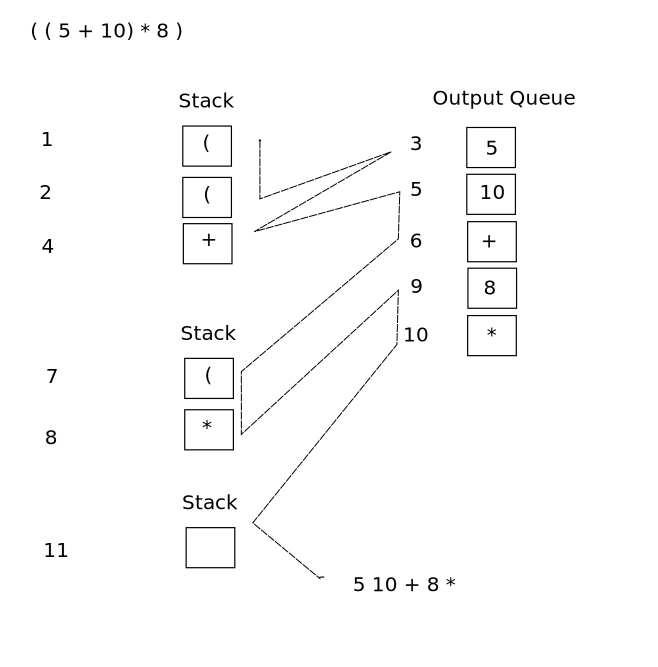
\includegraphics[scale=0.8]{images/shunting.png}
\caption{Shunting-yard Algorithm Example}
\label{fig:shunting}
\end{figure}

Now that the expression is in reverse Polish notation it is obvious the root node is "*" and it's children are "8" and "+". \\
As explained before there is a difference between arithmetic expressions and the compound diagram expression. So it is not necessary to check for operator precedence. Also the algorithm that is implemented here uses a vector instead of a queue because it is  much easier to deal with vectors than queues.

\subsubsection{Tree Building}
As stated earlier the rightmost operator is the root node in a postfix expression. Therefore in order to build the tree it is necessary to proceed from left to right to get all node objects instantiated properly before instantiating the root node. The tree building algorithm is as follows
\begin{itemize}
\item There is a node stack that holds nodes while  the parent and children.
\item Go through all nodes from left to right.
\item If a token is an operand (a diagram) 
\begin{enumerate}
\item Create a leaf node with the diagram as it's payload.
\item Push the node object onto the node stack.
\end{enumerate}

\item If the token is a binary operator i.e. $ \wedge , \vee $:
\begin{itemize}
\item If the token is the last token (it is the root):
\begin{enumerate}
\item Create the root node with the current token as it's payload.
\item Set the top of stack as it's left child.
\item Pop it from stack.
\item Set the top of stack as it's right child.
\item Pop from stack.
\end{enumerate}

\item Else
\begin{enumerate}
\item Create a node with the current token as it's payload.
\item Set the top of stack as it's left child.
\item Pop it from stack.
\item Set the top of stack as it's right child.
\item Pop from stack.
\item Push the node onto the stack.
\end{enumerate}

\end{itemize}
\item If the token is a unary operator i.e. $ \neg $:
\begin{itemize}
\item If the token is the last token (it is the root):
\begin{enumerate}
\item Create the root node with the current token ("NOT") as it's payload.
\item Set the top of stack as it's left child.
\item Pop it from stack.
\end{enumerate}

\item Else
\begin{enumerate}
\item Create a node with the current token ("NOT") as it's payload.
\item Set the top of stack as it's left child.
\item Pop it from stack.
\item Push the node onto the stack.
\end{enumerate}

\end{itemize}

\end{itemize}

In order to make the process easier to understand an example is provided to clarify the algorithm. The example below shows how the expression $( (d_{1} \wedge d_{2}) \vee ((d_{3} \wedge (\neg d_{4})) )  $ is made into a tree. The process of making the postfix expression is exactly the same as the example in figure (\ref{fig:shunting}) the only difference is that there is no checking for precedence. The postfix expression of this expression is $ d_{1} d_{2} \wedge d_{3} d_{4} \neg \wedge \vee $. The process of how the tree is built is provided in figure (\ref{fig:tree}) so the process can be observed visually. After the process is completed the tree is generated which is represented in figure (\ref{fig:tree2}).
 
\begin{figure}[h]
\centering
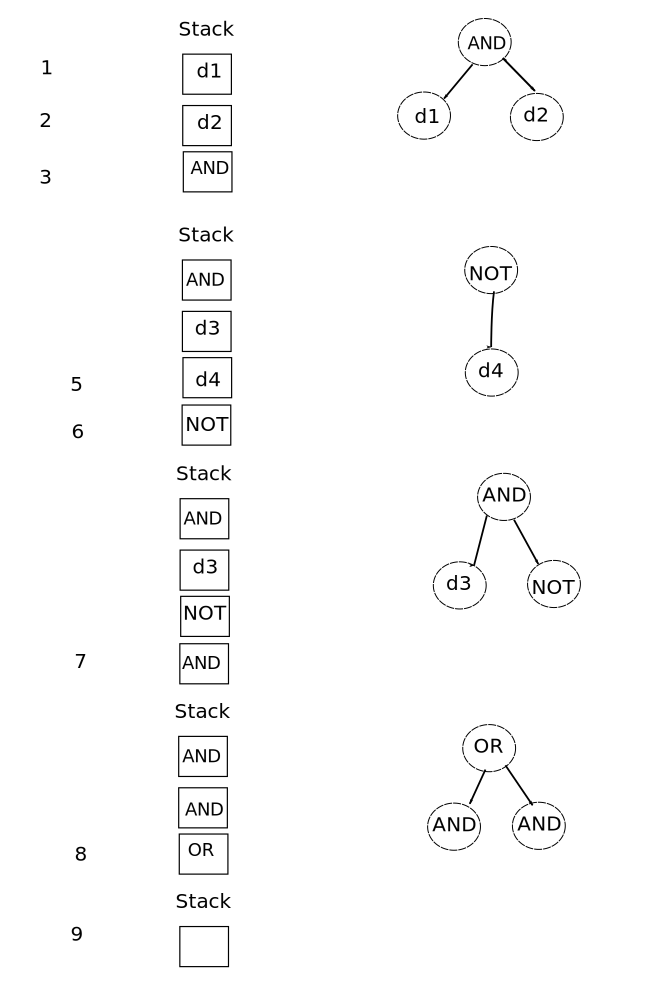
\includegraphics[scale=0.5]{images/tree.png}
\caption{Tree Building Process Example}
\label{fig:tree}
\end{figure}


\begin{figure}[h]
\centering
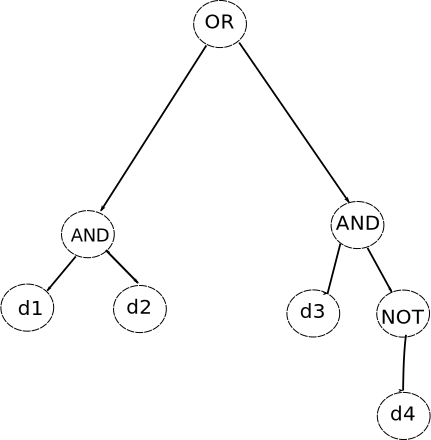
\includegraphics[scale=0.5]{images/tree2.png}
\caption{The Completed Tree}
\label{fig:tree2}
\end{figure}


\subsection{In-order Tree Traversal}
\label{inorder}
A traversal of a tree T is a systematic way of accessing, or visiting, all the nodes of T \cite{algo_book}. There are three different, well known, algorithms for traversing a tree which are listed below:
\begin{itemize}
\item Preorder: In preorder traversal of a tree T, the root of T is accessed first and then the sub trees rooted at its children are traversed recursively \cite{algo_book}. 
\item Postorder: This algorithm is the opposite of the preorder traversal, as it recursively traverses the sub trees rooted at the children of the root first, and then visits the root \cite{algo_book}.
\item Inorder: This traversal is for binary trees mainly. The way the algorithm works is that a node is visited between the recursive traversals of its left and right sub trees \cite{algo_book}.
\end{itemize}
For more details please refer to \cite{algo_book}.\\

After constructing a binary tree it is essential to develop an algorithm to be able to search the tree or to just re-construct the original expression. In this case it is necessary to implement an inorder tree traversal because it is required to visit each node in the same manner that the expression is read, from left to right. At this stage of the project, inorder traversal seems to be the only necessary algorithm for iterating through the expression tree, however, in the future there might be necessary to implement preorder or postorder algorithms as well. Because of this, a superclass Traversal is created so it can be extended in the future, if necessary. The figure (\ref{fig:traversal}) depicts inorder traversal in action and also algorithm below describes way inorder algorithm works:


\begin{itemize}
\item Start with the root node.

\item If node has left child:

\begin{itemize}
\item If node is a leaf:Do the necessary operation.
\item Else if the node is not a leaf recursively get the left node of the current node.
\end{itemize}

\item If node has right child:

\begin{itemize}
\item If node is a leaf:Do the necessary operation.
\item Else if the node is not a leaf recursively get the right node of the current node.
\end{itemize}

\item If node is a leaf: Do the necessary operations.
\end{itemize}

\begin{figure}[h]
\centering
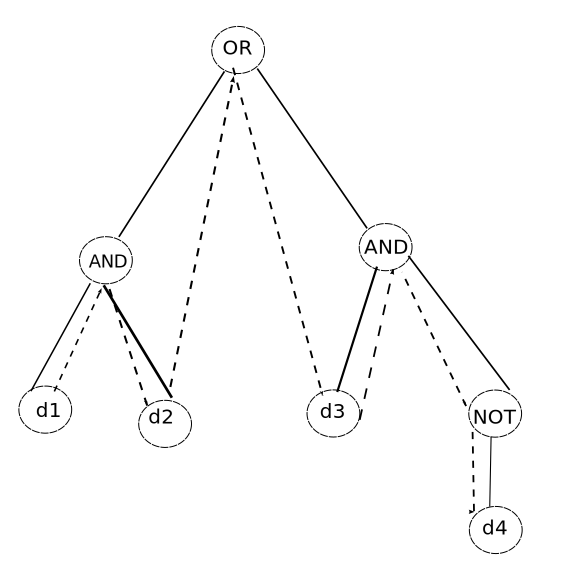
\includegraphics[scale=0.6]{images/inorder.png}
\caption{Inorder Tree Traversal}
\label{fig:traversal}
\end{figure}

The essence of the algorithm is that it recursively calls itself whenever it is visiting an internal node (any node of a tree that has child nodes and is thus not a leaf node) until it reaches a leaf node and then it starts to go upwards. After recursively reaching all the left nodes of the internal node, it recursively calls itself to reach the right leaf of the right child. By performing this operation recursively it can reach all nodes. The pseudo code of the algorithm and the actual C++ code of the algorithm are provided below:\\

Pseudo code:\\\\
\small
\begin{lstlisting}

inorder(CompoundNode *node): \\starts with the root node

	if node has a left child then
		inorder(left node)
		
	If node has a right child then
		inorder(right node)
				
\end{lstlisting}
\large
Implementation of the algorithm:\\\\

\small
\begin{lstlisting}
void InorderTraversal::traverse(CompoundNode *node)
{
  if (node->isLeaf())
	 cout << "Node Payload: " << node->getPayload().getLabel() << endl;
	 
  if (node->hasLeft())
    {
      if(node->isLeaf())
	{
	  cout << "Node Payload: " << node->getPayload().getLabel() << endl;
	}

      else if ( !node->isLeaf())
	{
	  traverse(node->getLeft()); \\recuresive call
	}
    }

  if(node->hasRight())
    {
      if(node->isLeaf())
	{
	  cout << "Node Payload: " << node->getPayload().getLabel() << endl;
	}

      else if ( !node->isLeaf())
	{
	  cout << "Getting the Right node: " << node->getType() << endl;
	  traverse(node->getRight());  \\recuresive call
	}
    }
}
					
\end{lstlisting}
\large

\subsection{Applying Rules}
In order to be able to apply a rule to a compound diagram, it is necessary to know whether it is possible to apply the rule, then, applying the rule. The method that can be used to check if a rule can be applied to a diagram is as follows:\\
Consider a rule i.e. DeMorgan's Law $ \neg (d_{1} \vee d_{2})$. The structure of this rule is drawn in a tree as shown in figure \ref{fig:dem}. It is clear from the picture that the operators Not and Or are in a specific order which means Not is the parent and Or is the child. All rules when are converted to postfix notation have the operators in a specific order which means if a compound diagram has the exact same pattern of operators (in the same order) it means that the rule can be applied to that diagram. The way this algorithm works for trying to apply a rule to a compound diagram is as described below:

\begin{figure}[h]
\centering
\includegraphics[scale=0.6]{images/dem.png}
\caption{DeMorgan's law's tree structure}
\label{fig:dem}
\end{figure}

\begin{itemize}
\item Get the predefined rule patten (the order in which the operators should be).
\item Iterate through the tree,
\item If the pattern is matched: it is possible to apply the rule.
\begin{enumerate}
\item Get the compound diagram's postfix notation.
\item Find the operators that match the pattern in the correct order.
\item Replace them as necessary.
\item Recreate the tree structure of the compound diagram.
\end{enumerate}
\end{itemize}

This method of checking if a rule is appliable and then applying it is done in the rules class. 

\newpage
\section{Testing}
\label{sec:Testing}
Testing is a process of technical investigation, performed on behalf of stakeholders, that is intended to reveal quality-related information about the product with respect to the context in which it is intended to operate \cite{testing_site}. This includes the process of running a program with the intent of finding errors. Testing can never prove the correctness of a piece of software completely: it can only provide some assurance for the customers and developers that the parts of the software that are tested, provide the functionality that is expected, in the context that they were tested. The process of creating error-free software applications requires technical sophistication in the analysis, design, and implementation of that software and proper test planning, as well as robust automated testing tools \cite{ISTQB_book}.\\

There testing methods that are used in this project are:
\begin{itemize}
\item Black-Box Testing
\item Unit Testing
\end{itemize}

As explained earlier there are two parts in this project:
\begin{itemize}
\item Unitary Prover 
\item Compound Prover
\end{itemize}
which both have different strategies towards testing. The first part which is the unitary prover, was mostly tested based on Black-Box testing strategy as it was not as complex as the compound part. The implementation of the second part of the project was mostly done by unit tests which were written for each specific component. Similar to other sections of this project, lack of understating of testing and its use before starting to test, was the reason why other methods of testing were not used. For instance white-box (the method that tests every single path in the program) testing could have been used in situations where knowing how the program behaves under different circumstances was important or test driven development (which the programmer writes the test before implementing the class to reduce misunderstandings in the requirement and know exactly what should each function do) could have been helpful  because it helps the programmer understand what each function should do before starting to implement them and therefore reduce the possibility of mistakes during implementation. However, as stated earlier because of lack of understanding and limited time, more elaborate methods of testing were not applied. How this project was tested is explained in later sections. 

\subsection{Black-Box Testing}
Black box testing is a method of testing which treats the software as a "black box" without any knowledge of how its internal components work \cite{ISTQB_book}. In this method the tester inputs valid and invalid input to the program and observes the behaviour of the software. If the desired results are not produced, it means that there is a bug which has to be fixed. The advantages of black-box testing are:
\begin{itemize}
\item It is more effective on larger units of code compared to white-box testing.
\item Tester needs no knowledge of the implementation of the software.
\item The programmer and tester can be independent from each other.
\item Tests are done in a way as if the user is using the system.
\item Tests can be prepared when the specification is completed.
\item It is faster compared to white-box testing.
\end{itemize}

There a number of disadvantages as well which are:
\begin{itemize}
\item It is possible to only test a small number of inputs. It is impossible to test everything.
\item Without unambiguous specification, it is hard to design the tests because the tester does not know exactly what is the output of each input supposed to be.
\item May leave many possible program paths untested.
\end{itemize}
For more details refer to \cite{ISTQB_book} and \cite{blackbox_site}. The advantages that black-box testing has made it a suitable choice for a testing strategy for this project. The way black-box testing is used, is explained in section \ref{unitary_testing}.

\subsection{Unit Testing}
Unit testing tests a small software unit at a time, which is typically performed by the individual programmer who implemented the unit. Depending on the different programming
languages used, this unit may test a function, a procedure, or a subroutine in traditional programming languages such as C or PASCAL, or a method in object-oriented languages such as C++ or Java. In unit testing usually the main focus is the implementation details which is normally used with white-box testing \cite{unittesting_book}. It is not always necessary to use white-box testing on each unit, it is possible to use black-box testing on each method as well. For instance, it is possible to test a method only by passing it the parameters it needs and check whether or not it produces the desired output \cite{unittesting_book}. Of course it does not prove anything that the method is correct but it provides satisfactory evidence for the time begin that the method works. For more details on unit testing please refer to \cite{unittesting_book}.\\
There are a great deal of reasons why to use unit tests, some of them are listed below:

\begin{itemize}
\item Unit testing is a documentation for the system because programmers can have a look at each unit test to understand what each unit does and how it can be used.
\item Unit tests that are used in test-driven development can take the place of formal design because each unit test can be treated as an element which describes what each class is supposed to do.
\item Code refactoring becomes easier because if a module changes and causes a problem it can be quickly identified and fixed. After refactoring if the unit test passes, it means that the system is still working as the unit test expects it.
\end{itemize}
For more detail on unit tests refer to \cite{KentBeck_site}.\\

Clearly using unit testing is an acceptable choice of testing because it is logical to divide testing process into smaller, manageable units that can provide the assurance that each small unit works properly. Obviously for large projects the number of unit tests that are required is significantly enormous and it will be very difficult to manage that great deal of unit tests. Because of this issue there are a number of frameworks that are provided to manage and run unit tests automatically which are remarkably helpful in the process of testing. One of the most well-known testing frameworks is JUnit which is for Java programs. It provides an environment for tests to be written in and then are automatically compiled and run by JUnit and at the end of the process it informs the tester whether or not a test filled. \\

As this project is written in C++, JUit was not possible to be used and it was necessary to use a framework that can be used with C++ code. The framework that is used in this project is CPPUnit which is like JUnit but it is for C++.

\subsection{Unitary Theorem Proving Testing}
\label{unitary_testing}
The unitary diagram theorem prover is tested using black-box strategy which is testing the functionality of the system as a whole. As it is depicted in figure (\ref{fig:blackBox}) the black-box is the prover, the inputs are different diagram files and the output is the produced proofs.

\begin{figure}[h]
\centering
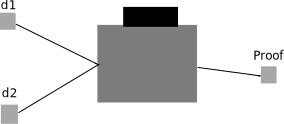
\includegraphics[scale=1.0]{images/blackbox.png}
\caption{Black Box Testing}
\label{fig:blackBox}
\end{figure}

Applying black-box testing was done as follows:
\begin{enumerate}
\item Create a number of different unitary diagrams.
\item Write the proof manually for at least 10 different pairs of diagrams.
\item Test each one of them with the program.
\item If they all produce the correct answer, it seems the program is behaving correctly.
\end{enumerate}

The disadvantage with this method was that it was very time consuming and difficult to perform the tests as no automation was done. It would have made much more sense if the tests were automated and black-box testing would have been used with unit tests.\\

\subsubsection{Tested Diagrams}
The diagrams that were produced for testing this part of the project are represented in figure (\ref{fig:testDiagrams}).

\begin{figure}[]
\centering
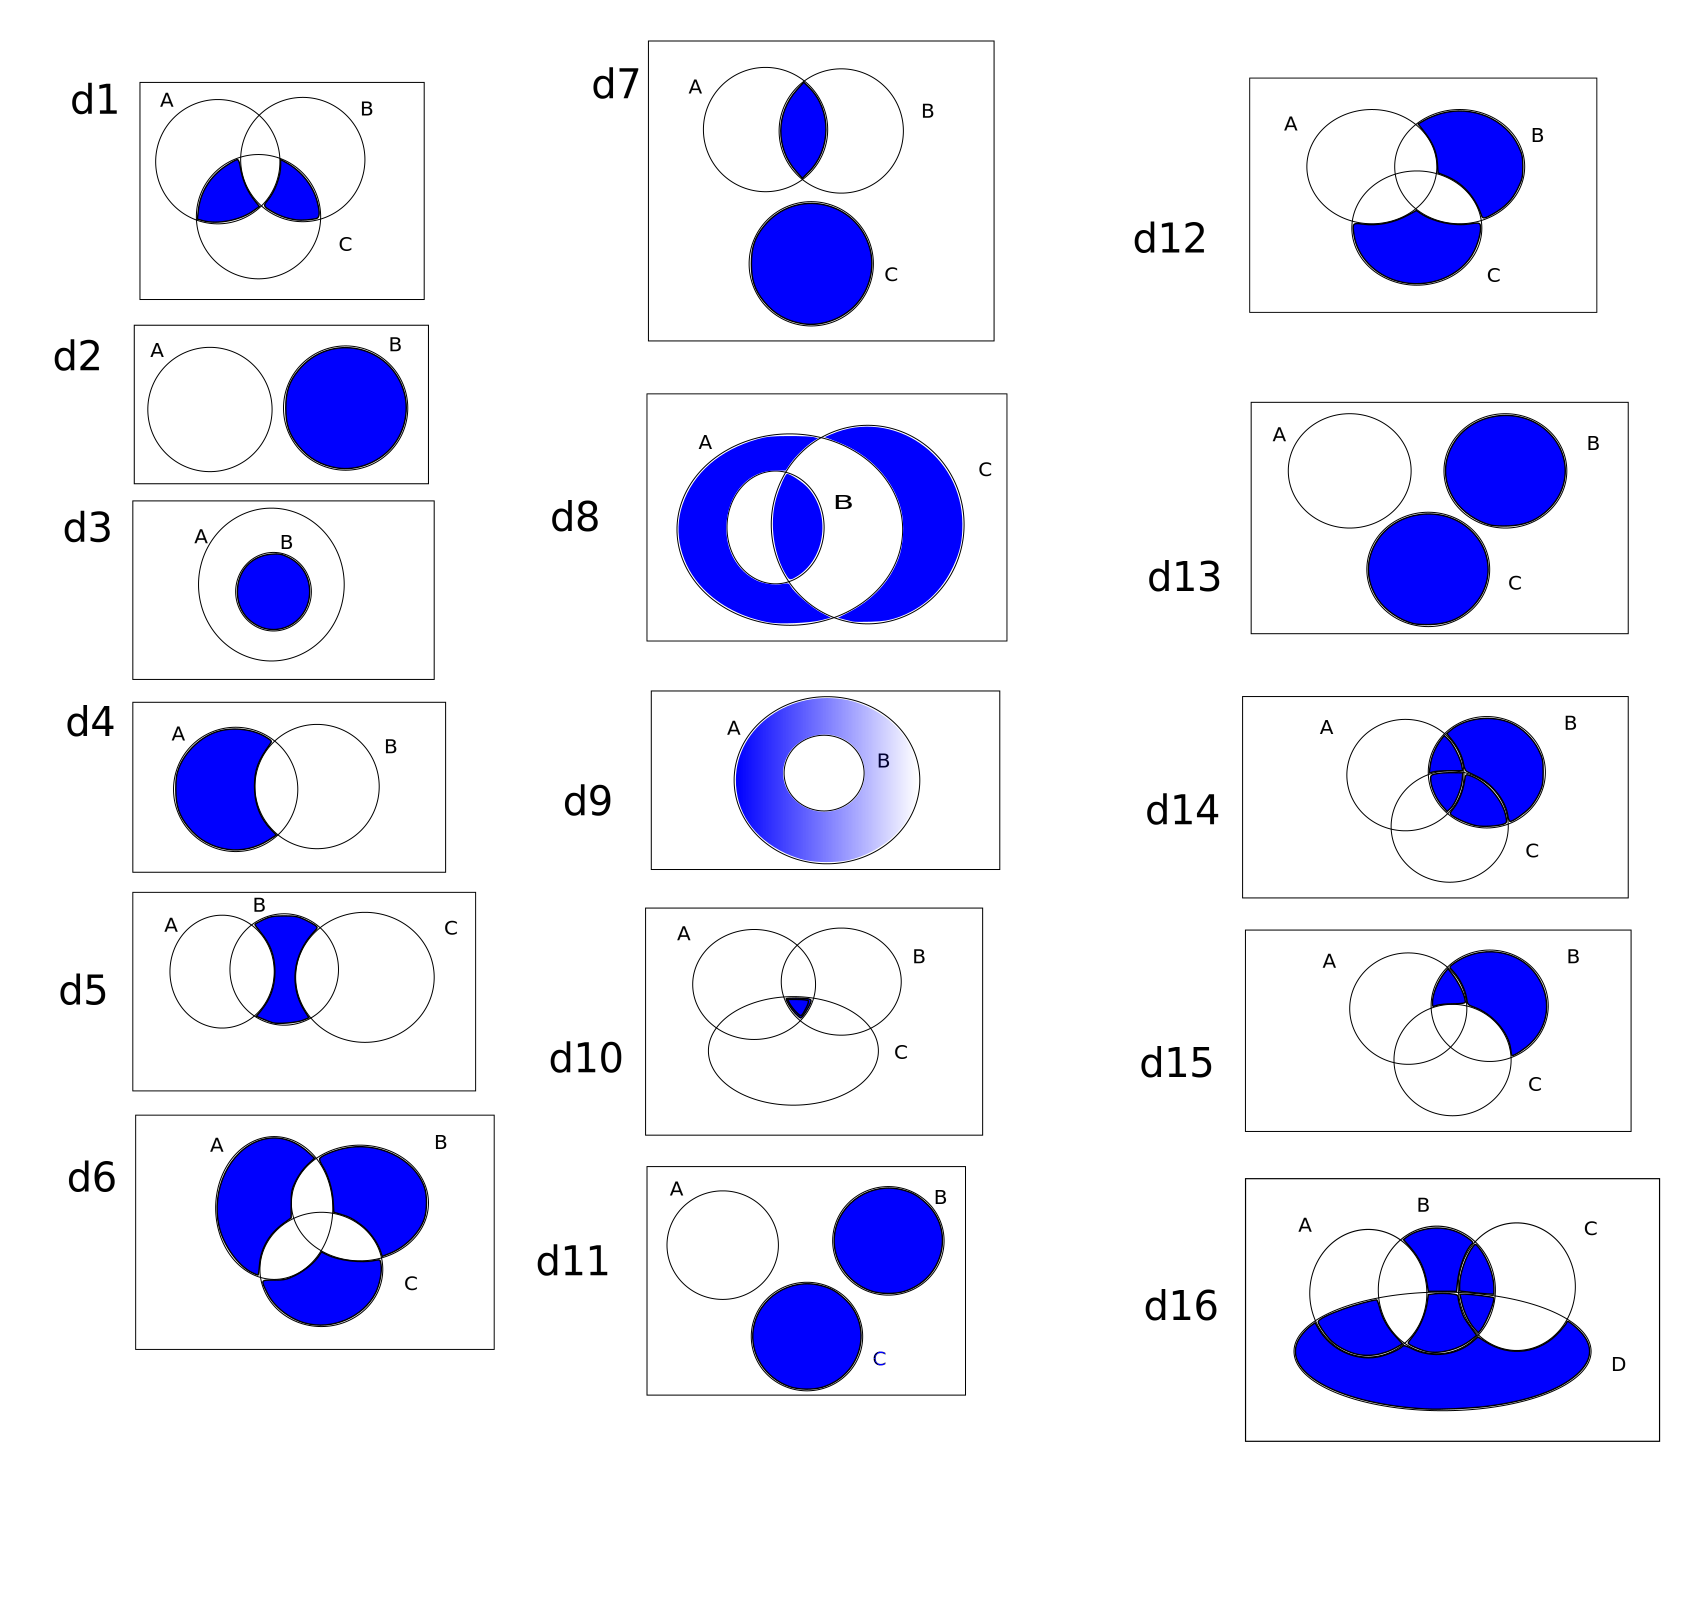
\includegraphics[scale=0.5]{images/allDiagrams.png}
\caption{Test Diagrams}
\label{fig:testDiagrams}
\end{figure}

Some tests are provided in sections below so it can be observed how the process of testing works.

\subsubsection{Test 1: $ d_{7} \rightarrow  d_{1} $}
Testing to see if $ d_{7} $ follows from $ d_{1} $ is represented below and demonstrated with screenshots of the program. The abstract syntax of the diagram from file "d1" is:
\small
\begin{lstlisting}
label = d1;
contours      = {A, B, C};
zones		  = {(A,BC) , (BC,A), (B,AC),(C,AB), (AB,C) , (AC, B), (ABC, ), ( , ABC) };
shaded-zones  = {(AC, B), (BC,A)};					
\end{lstlisting}
\large

and for file "d7" is:

\small
\begin{lstlisting}
label = d7;
contours      = {A, B, C};
zones		  = {(A,BC) ,(B,AC),(C,AB), (AB,C), ( , ABC) };
shaded-zones  = { (AB,C) , (C,AB) };					
\end{lstlisting}
\large

\begin{enumerate}
\item No zone is missing from $ d_{1} $. No action required.
\item Zones $ (AC,B), (BC,A), (ABC, ) $ are missing from $ d_{7} $ which are needed to be added. The new diagram is called $ d^sh_{7} $.
\item Now the shaded zones in $ d^sh_{7} $ are $ \lbrace (AC,B), (BC,A), (ABC, ), (AB,C), (C,AB) \rbrace $.
\item There are no missing contours.
\item It is clear that all $ d_{1} $ shaded zones are a subset of $ d^sh_{7} $ which means a proof exists.
\item But a proof from $ d_{1} $ to $ d_{7} $ does not exist as not all shaded zones from $ d^sh_{7} $ exists in $ d_{1} $. So $ d_{1} \nrightarrow d_{7} $.
\end{enumerate}

The series of screen shots that are provided below demonstrate how the program can be used to prove that there is a proof from $ d_{7} \rightarrow d_{1} $.

\begin{figure}[h]
\centering
\includegraphics[scale=0.7]{images/ss1.png}
\caption{Loading diagrams into the program}
\label{fig:loading}
\end{figure}

\begin{figure}[h]
\centering
\includegraphics[scale=0.7]{images/ss2.png}
\caption{Running "prove" command}
\label{fig:prove}
\end{figure}

Note that the diagram details that are shown in the "command line" in figure (\ref{fig:proved}) are not part of the proof. They are just there to show the user what the program is currently doing. If a proof exists, a message will be shown that a proof exists and then it is saved in the file called "proof.txt" in the current folder (where the executable file of the program is).\\


\begin{figure}[h]
\centering
\includegraphics[scale=0.5]{images/ss3.png}
\caption{Running the proof algorithm and generating the "proof.txt" file}
\label{fig:proved}
\end{figure}

The generated proof that is saved in "proof.txt" is demonstrated below:

\small
\begin{lstlisting}
Genrated Proof:
------------------------------------------------------
Label: d7

Contours: { A , B , C } 

Selected Zones: { (A , BC) , (B , AC) , (C , AB) , (AB , C) , ( , ABC) }  

ShadedZones: { (AB , C) , (C , AB) } 


------------------------------------------------------
Label: d7-ASZ-ASZ-ASZ

Contours: { A , B , C } 

Selected Zones: { (A , BC) , (B , AC) , (C , AB) , (AB , C) , ( , ABC) , (AC , B) , (BC , A) , (ABC , ) }  

ShadedZones: { (AB , C) , (C , AB) , (AC , B) , (BC , A) , (ABC , ) } 


------------------------------------------------------
Label: d7-ASZ-ASZ

Contours: { A , B , C } 

Selected Zones: { (A , BC) , (B , AC) , (C , AB) , (AB , C) , ( , ABC) , (AC , B) , (BC , A) }  

ShadedZones: { (AB , C) , (C , AB) , (AC , B) , (BC , A) } 


------------------------------------------------------
Label: d7-ASZ

Contours: { A , B , C } 

Selected Zones: { (A , BC) , (B , AC) , (C , AB) , (AB , C) , ( , ABC) , (AC , B) }  

ShadedZones: { (AB , C) , (C , AB) , (AC , B) } 


------------------------------------------------------
Label: d1

Contours: { A , B , C } 

Selected Zones: { (A , BC) , (BC , A) , (B , AC) , (C , AB) , (AB , C) , (AC , B) , (ABC , ) , ( , ABC) }  

ShadedZones: { (AC , B) , (BC , A) } 
\end{lstlisting}
\large

\subsubsection{Test 2: $ d_{4} \nrightarrow  d_{10} $}
This test is provided to test the absence of a proof for diagrams $ d_{4} $ and $ d_{10} $. Note that only the final screenshot is provided to show the final result. The abstract syntax of $ d_{4} $ is:

\small
\begin{lstlisting}
label = d4;
contours      = {A, B};
zones		= {(AB, ),(A,B), (B,A), ( , AB) };
shaded-zones  = { ( A , B ) };
\end{lstlisting}
\large

and the abstract syntax of $ d_{10} $ is:

\small
\begin{lstlisting}
label = d10;
contours      = {A, B, C};
zones		= {(A,BC) ,(B,AC),(C,AB), (AB,C), (AC, B) , (BC, A), (ABC, ), ( , ABC) };
shaded-zones  = { (ABC, ) };
\end{lstlisting}
\large

\begin{enumerate}
\item No missing zones are needed to be added to $ d_{4} $.
\item No missing zones are needed to be added to $ d_{10} $.
\item Adding missing contour "C" to $ d_{4} $. The resulting diagram is called $ d^L_{4} $.
\item Now the abstract syntax of the diagram $ d^L_{4} $ is:
\small
\begin{lstlisting}
contours      = {A, B, C};
zones		= {(A,BC) ,(B,AC),(C,AB), (AB,C), (AC, B) , (BC, A), (ABC, ), ( , ABC) };
shaded-zones  = {(A,BC), (AC, B)};
\end{lstlisting}
\large
\item Because the shaded zone in $ d_{10} $ is not a subset of the shaded zones in $ d_{4} $ there is no proof for these two diagrams.
\end{enumerate}  

The screen-shot of the result of this test is provided in figure (\ref{fig:test2}).

\begin{figure}[h]
\centering
\includegraphics[scale=0.5]{images/ss4.png}
\caption{Proving $  d_{4} \rightarrow d_{10} $ : No proof exists}
\label{fig:test2}
\end{figure}

\subsubsection{Test 3: $ d_{6} \nrightarrow  d_{5} $}
There is no proof for $ d_{6} \rightarrow  d_{5} $ or $ d_{5} \rightarrow  d_{6} $. The process is shown below:\\

The abstract syntax of $d _{5} $:
\small
\begin{lstlisting}
label = d5;
contours      = {A, B, C};
zones		= {(A,BC) ,(B,AC),(C,AB), (AB,C) , (BC, A),  ( , ABC) };
shaded-zones  = { (B,AC) };
\end{lstlisting}
\large

and the abstract syntax of $ d_{6} $ is:

\small
\begin{lstlisting}
label = d6;
contours      = {A, B, C};
zones		= {(A,BC) ,(B,AC),(C,AB), (AB,C), (AC, B) , (BC, A), (ABC, ), ( , ABC) };
shaded-zones  = { (A,BC) ,(B,AC),(C,AB) };
\end{lstlisting}
\large

\begin{enumerate}
\item No missing zones are needed to be added to $ d_{6} $.
\item Missing zones $ (AC , B) , (ABC , )  $ are needed to be added to $ d_{5} $. The resulting diagram is called $ d^sh_{5} $.
\item There are no missing contours in either diagrams.
\item Because the shaded zone in $ d^sh_{5} $ is not a subset of the shaded zones in $ d_{6} $ there is no proof for these two diagrams.
\end{enumerate}  

The screenshot of the result of this test is provided in figure (\ref{fig:test3}). Also to depict that $  d_{5} \rightarrow d_{6} $ does not follow, the result screenshot is represented in figure (\ref{fig:test4}).

\begin{figure}[h]
\centering
\includegraphics[scale=0.4]{images/ss5.png}
\caption{Proving $  d_{6} \rightarrow d_{5} $ : No proof exists}
\label{fig:test3}
\end{figure}


\begin{figure}[h]
\centering
\includegraphics[scale=0.4]{images/ss6.png}
\caption{Proving $  d_{5} \rightarrow d_{6} $ : No proof exists}
\label{fig:test4}
\end{figure}

\subsubsection{Test 4: $ d_{13} \rightarrow  d_{12} $}

The abstract syntax of $d _{12} $:
\small
\begin{lstlisting}
label = d12;
contours      = {A, B, C};
zones		= {(A,BC) ,(B,AC),(C,AB), (AB,C), (AC, B) , (BC, A), (ABC, ), ( , ABC) };
shaded-zones  = { (B,AC),(C,AB) };
\end{lstlisting}
\large

and the abstract syntax of $ d_{13} $ is:

\small
\begin{lstlisting}
label = d13;
contours      = {A, B, C};
zones		= {(A,BC) ,(B,AC),(C,AB), ( , ABC) };
shaded-zones  = { (B,AC),(C,AB) };
\end{lstlisting}
\large

\begin{enumerate}
\item Missing zones $ (AB,C), (AC, B) , (BC, A), (ABC, ) $ are needed to be added to $ d_{13} $. The resulting diagram is called $ d^sh_{13} $. The abstract syntax of the diagram is represented below:
\small
\begin{lstlisting}
Label: d13-ASZ-ASZ-ASZ-ASZ
Contours: { A , B , C } 
Selected Zones: { (A , BC) , (B , AC) , (C , AB) , ( , ABC) , (AB , C) , (AC , B) , (BC , A) , (ABC , ) }  
ShadedZones: { (B , AC) , (C , AB) , (AB , C) , (AC , B) , (BC , A) , (ABC , ) } 
\end{lstlisting}
\large
\item No action is necessary to be done on $ d_{12} $.
\item There are no missing contours in either diagrams.
\item Because the shaded zone in $ d_{12} $ are all shaded in $ d^sh_{13} $ as well, there is a proof for these two diagrams.
\end{enumerate}  

The screenshot of the result of this test is provided in figure (\ref{fig:test5}). The proof from the file "proof.txt" is also shown below:

\small
\begin{lstlisting}
------------------------------------------------------
Label: d13

Contours: { A , B , C } 

Selected Zones: { (A , BC) , (B , AC) , (C , AB) , ( , ABC) }  

ShadedZones: { (B , AC) , (C , AB) } 


------------------------------------------------------
Label: d13-ASZ-ASZ-ASZ-ASZ

Contours: { A , B , C } 

Selected Zones: { (A , BC) , (B , AC) , (C , AB) , ( , ABC) , (AB , C) , (AC , B) , (BC , A) , (ABC , ) }  

ShadedZones: { (B , AC) , (C , AB) , (AB , C) , (AC , B) , (BC , A) , (ABC , ) } 


------------------------------------------------------
Label: d13-ASZ-ASZ-ASZ

Contours: { A , B , C } 

Selected Zones: { (A , BC) , (B , AC) , (C , AB) , ( , ABC) , (AB , C) , (AC , B) , (BC , A) }  

ShadedZones: { (B , AC) , (C , AB) , (AB , C) , (AC , B) , (BC , A) } 


------------------------------------------------------
Label: d13-ASZ-ASZ

Contours: { A , B , C } 

Selected Zones: { (A , BC) , (B , AC) , (C , AB) , ( , ABC) , (AB , C) , (AC , B) }  

ShadedZones: { (B , AC) , (C , AB) , (AB , C) , (AC , B) } 


------------------------------------------------------
Label: d13-ASZ

Contours: { A , B , C } 

Selected Zones: { (A , BC) , (B , AC) , (C , AB) , ( , ABC) , (AB , C) }  

ShadedZones: { (B , AC) , (C , AB) , (AB , C) } 


------------------------------------------------------
Label: d12

Contours: { A , B , C } 

Selected Zones: { (A , BC) , (B , AC) , (C , AB) , (AB , C) , (AC , B) , (BC , A) , (ABC , ) , ( , ABC) }  

ShadedZones: { (B , AC) , (C , AB) } 
\end{lstlisting}
\large


\begin{figure}[h]
\centering
\includegraphics[scale=0.4]{images/ss7.png}
\caption{Proving $  d_{13} \rightarrow d_{12} $ : Proof exists}
\label{fig:test5}
\end{figure}

\subsubsection{Test 5: $ d_{16} \rightarrow  d_{5} $}

The abstract syntax of $d _{16} $:
\small
\begin{lstlisting}
label 		  = d16;
contours      = {A, B, C, D};
zones		  = {( , ABCD) , (A , BCD) , (B , ACD) , (C , ABD) , (D , ABC) , (AB , CD) ,  (AD , BC) , (BC , AD) , (BD , AC) , (CD , AB) , (ABD , C) ,  (BCD , A)  };
shaded-zones  = {(B , ACD) , (D , ABC) , (AD , BC) , (BC , AD) , (BD , AC) , (BCD , A)};
\end{lstlisting}
\large

and the abstract syntax of $ d_{5} $ is:

\small
\begin{lstlisting}
label = d5;
contours      = {A, B, C};
zones		= {(A,BC) ,(B,AC),(C,AB), (AB,C) , (BC, A),  ( , ABC) };
shaded-zones  = { (B,AC) };
\end{lstlisting}
\large

\begin{enumerate}
\item Missing zones $ (AC , BD) , (ABC , D) , (ACD , B) , (ABCD , ) $ are needed to be added to $ d_{16} $. The resulting diagram is called $ d^sh_{16} $.
\item Missing zones $ (AC , B) , (ABC , )  $ are needed to be added to $ d_{5} $. The resulting diagram is called $ d^sh_{5} $.
\item The missing contour "D" is added to $ d_{5} $. The resulting diagram is called $ d^L_{5} $.
\item Because the shaded zone in $ d^L_{5} $ is a subset of shaded zones in $ d^sh_{16} $, there is a proof for these two diagrams.
\end{enumerate}  

The screenshot of the result of this test is provided in figure (\ref{fig:test6}). The proof from the file "proof.txt" is also shown below:

\small
\begin{lstlisting}
------------------------------------------------------
Label: d16

Contours: { A , B , C , D } 

Selected Zones: { ( , ABCD) , (A , BCD) , (B , ACD) , (C , ABD) , (D , ABC) , (AB , CD) , (AD , BC) , (BC , AD) , (BD , AC) , (CD , AB) , (ABD , C) , (BCD , A) }  

ShadedZones: { (B , ACD) , (D , ABC) , (AD , BC) , (BC , AD) , (BD , AC) , (BCD , A) } 


------------------------------------------------------
Label: d16-ASZ-ASZ-ASZ-ASZ

Contours: { A , B , C , D } 

Selected Zones: { ( , ABCD) , (A , BCD) , (B , ACD) , (C , ABD) , (D , ABC) , (AB , CD) , (AD , BC) , (BC , AD) , (BD , AC) , (CD , AB) , (ABD , C) , (BCD , A) , (AC , BD) , (ABC , D) , (ACD , B) , (ABCD , ) }  

ShadedZones: { (B , ACD) , (D , ABC) , (AD , BC) , (BC , AD) , (BD , AC) , (BCD , A) , (AC , BD) , (ABC , D) , (ACD , B) , (ABCD , ) } 


------------------------------------------------------
Label: d16-ASZ-ASZ-ASZ

Contours: { A , B , C , D } 

Selected Zones: { ( , ABCD) , (A , BCD) , (B , ACD) , (C , ABD) , (D , ABC) , (AB , CD) , (AD , BC) , (BC , AD) , (BD , AC) , (CD , AB) , (ABD , C) , (BCD , A) , (AC , BD) , (ABC , D) , (ACD , B) }  

ShadedZones: { (B , ACD) , (D , ABC) , (AD , BC) , (BC , AD) , (BD , AC) , (BCD , A) , (AC , BD) , (ABC , D) , (ACD , B) } 


------------------------------------------------------
Label: d16-ASZ-ASZ

Contours: { A , B , C , D } 

Selected Zones: { ( , ABCD) , (A , BCD) , (B , ACD) , (C , ABD) , (D , ABC) , (AB , CD) , (AD , BC) , (BC , AD) , (BD , AC) , (CD , AB) , (ABD , C) , (BCD , A) , (AC , BD) , (ABC , D) }  

ShadedZones: { (B , ACD) , (D , ABC) , (AD , BC) , (BC , AD) , (BD , AC) , (BCD , A) , (AC , BD) , (ABC , D) } 


------------------------------------------------------
Label: d16-ASZ

Contours: { A , B , C , D } 

Selected Zones: { ( , ABCD) , (A , BCD) , (B , ACD) , (C , ABD) , (D , ABC) , (AB , CD) , (AD , BC) , (BC , AD) , (BD , AC) , (CD , AB) , (ABD , C) , (BCD , A) , (AC , BD) }  

ShadedZones: { (B , ACD) , (D , ABC) , (AD , BC) , (BC , AD) , (BD , AC) , (BCD , A) , (AC , BD) } 


------------------------------------------------------
Label: d5-ASZ-ASZ-AC

Contours: { A , B , C , D } 

Selected Zones: { (A , BCD) , (AD , BC) , (B , ACD) , (BD , AC) , (C , ABD) , (CD , AB) , (AB , CD) , (ABD , C) , (BC , AD) , (BCD , A) , ( , ABCD) , (D , ABC) , (AC , BD) , (ACD , B) , (ABC , D) , (ABCD , ) }  

ShadedZones: { (B , ACD) , (BD , AC) , (AC , BD) , (ACD , B) , (ABC , D) , (ABCD , ) } 


------------------------------------------------------
Label: d5-ASZ-ASZ

Contours: { A , B , C } 

Selected Zones: { (A , BC) , (B , AC) , (C , AB) , (AB , C) , (BC , A) , ( , ABC) , (AC , B) , (ABC , ) }  

ShadedZones: { (B , AC) , (AC , B) , (ABC , ) } 


------------------------------------------------------
Label: d5-ASZ

Contours: { A , B , C } 

Selected Zones: { (A , BC) , (B , AC) , (C , AB) , (AB , C) , (BC , A) , ( , ABC) , (AC , B) }  

ShadedZones: { (B , AC) , (AC , B) } 


------------------------------------------------------
Label: d5

Contours: { A , B , C } 

Selected Zones: { (A , BC) , (B , AC) , (C , AB) , (AB , C) , (BC , A) , ( , ABC) }  

ShadedZones: { (B , AC) } 
\end{lstlisting}
\large


\begin{figure}[h]
\centering
\includegraphics[scale=0.4]{images/ss8.png}
\caption{Proving $  d_{16} \rightarrow d_{5} $ : Proof exists}
\label{fig:test6}
\end{figure}

All these five tests where provided to demonstrate how the testing phase for "unitary prover" part of the project was done. More tests have been performed as well but in order to save space they are not added to this documentation. Overall strategy of all the tests is the same, the only difference is what diagrams have been used to be tested. 

\subsection{Compound Diagram Phase Testing}
The lessons that were learnt about testing from the first part of the project made the choice of using unit tests an essential necessity. Having to manually run the tests every time a change has been made was a very time consuming task and as the second part of the project is relatively larger than the first part, it is crucial to save as much time as possible and automate as many tasks as possible. Therefore the implementation of the second part of the project was done by using unit tests with CPPUnit framework. In the subsections below the unit test for each component is provided and explained. It is important to note that all the unit tests perform testing based on black-box testing strategy which means that they test the functionality of the class as a whole to ensure that it fulfils the responsibility it was assigned to, but they do not test every single function in the class individually.     

\subsubsection{Unit Test 1: ExpressionTokenizer}
The responsibility of the ExpressionTokenizer is to tokenize a given compound diagram expression and return a vector of string tokens. The unit test for this class is provided below.
\small
\begin{lstlisting}
#include "ExpressionTokenizerTest.h"

CPPUNIT_TEST_SUITE_REGISTRATION (ExpressionTokenizerTest);

void ExpressionTokenizerTest::setUp()
{
  e = "(d1 and d2) and not d3"; //string expression
}

void ExpressionTokenizerTest::expressionTokenizerTest()
{
  ExpressionTokenizer *tokenizer = new ExpressionTokenizer (e);
  tokens =   tokenizer->tokenize();

  cout<< "\n Displaying tokens" << endl;   
  tokenizer->displayTokens(); //print all tokens

  CPPUNIT_ASSERT(tokens.size() > 0); //assert the size of tokens is greater than zero
}
\end{lstlisting}
\large

This unit test although simple but tests whether or not the expression was tokenized and by displaying the tokens it is possible to check that tokens are tokenized properly. Of course it is possible to make the test more elaborate but because of the simplicity of the task it was not necessary to test the output more. However, it is possible to test that all tokens that are returend are matched with the actual tokens in expression.
  
\subsubsection{Unit Test 2: InfixToPostfix}
The task of this class is to get the tokens and convert the given expression which is in infix notation to postfix notation. In the set-up function the necessary objects are instantiated and then the test is run. In this unit test the last node that is returned by InfixToPostfix is checked to be a "NOT" node. If it is, there is a high probability that this class has done its job correctly. The code for this test is represented below:
  
\small
\begin{lstlisting}
#include "InfixPostfixTest.h"
CPPUNIT_TEST_SUITE_REGISTRATION (InfixPostfixTest);

void InfixPostfixTest::setUp()
{
  //d1 d2 and d3 not and not ---> postfix
  e = "not( (d1 and d2) and (not d3))";
  
  ExpressionTokenizer *tokenizer = new ExpressionTokenizer(e);
  tokens = tokenizer->tokenize();
}

void InfixPostfixTest::infixPostfixTest()
{
  InfixToPostfix *infix2post = new InfixToPostfix (tokens);
  cout << "Displaying  Postfix: " << endl;
  
  infix2post->displayPostfix();
  vector<string> postfix =  infix2post->getPostfix();
  
  CPPUNIT_ASSERT(postfix.size() > 0);

  //the last node is a NOT node for this expression, check it
  CPPUNIT_ASSERT(postfix[postfix.size() -1] == "NOT" );
}
\end{lstlisting}
\large

\subsubsection{Unit Test 3: CompoundNode}
Before starting the implementation of the TreeBuilder it is necessary to be certain that the CompoundNode class works correctly. So the test below was written to ensure that this class performs its primitive functionality properly.

\small
\begin{lstlisting}
#include "CompoundNodeTest.h"


CPPUNIT_TEST_SUITE_REGISTRATION (CompoundNodeTest);

void CompoundNodeTest::setUp()
{
  p = new CompoundNode("AND", true);
  n1 = new CompoundNode(p, "and");
  n2 = new CompoundNode(p, "and");
  a = new CompoundNode(d1,"leaf d1");
  b = new CompoundNode(d2,"leaf d2");
  c = new CompoundNode(d3,"leaf d3");
  d = new CompoundNode(d4,"leaf d4");
  
  dEmpty.setLabel("empty");
  d1.setLabel("d1");
  d2.setLabel("d2");
  d3.setLabel("d3");
  d4.setLabel("d4");
}

void CompoundNodeTest::tearDown()
{

}

void CompoundNodeTest::compoundNodeTest()
{
   
  p->setLeft(n1);
  p->setRight(n2);
  n1->setLeft(a);
  n1->setRight(b);
  n2->setLeft(c);
  n2->setRight(d);
  
  cout << "\n" << p->getType() << p->isRoot() << endl;
  cout << "Roots Left: " << p->getLeft()->getType() << endl;
  cout << "Roots Right: " << p->getRight()->getType() << endl;

  cout << "R->Left->Left: " << p->getLeft()->getLeft()->getType() << endl;
  cout << "R->Left->Left: " << p->getLeft()->getRight()->getType() << endl;
  cout << "R->Right->Left  : " << p->getRight()->getLeft()->getType() << endl;
  cout << "R->Right->Right : " << p->getRight()->getRight()->getType() << endl;
  cout << n1->getType() << endl;
  cout << n2->getType() << endl;
  cout << a->getType() << endl;
  cout << b->getType() << endl;
  cout << c->getType() << endl;
  cout << d->getType() << endl;
  
  CPPUNIT_ASSERT (p->hasLeft() == true);
  CPPUNIT_ASSERT (p->hasRight() == true);
}
\end{lstlisting}
\large

The test succeeds which means setting the left and right children of a node works as expected. 

\subsubsection{Unit Test 4: TreeBuilder}
This class is responsible for constructing a tree object. The task of creating a tree object is an important task which needs more elaborate testing compared to the previous tests. The test for this class is first creating a compound diagram expression and, then, building the tree for it by running the "builder" function of TreeBuilder class and then checking whether the root node is correct and it carries the right payload. Also checking to ensure that the CompoundTree object's nodes are not empty means that the nodes are set in the object.
\small
\begin{lstlisting}
#include "TreeBuilderTest.h"
CPPUNIT_TEST_SUITE_REGISTRATION (TreeBuilderTest);

void TreeBuilderTest::setUp()
{
  e = "(../d/d1 and ../d/d2) and (../d/d3 or ../d/d4)"; //expression
}
void TreeBuilderTest::treeBuilderTest()
{

  cout << "\nStarting Tree Builder..."  << endl;
  TreeBuilder builder(e);
  builder.build();
  cout <<"Building Ended..." << endl;
  CompoundTree tree = builder.getTree();

  CompoundNode *root = tree.getRoot();

  cout << "Root  Node:  " << root->getType() << endl;
  
  CPPUNIT_ASSERT(root->getType().size() > 0);
  CPPUNIT_ASSERT(tree.getNodes().size() > 0);
}
\end{lstlisting}
\large

\subsubsection{Unit Test 5: TreeTraversal}
This class is tested by creating a tree based on a defined expression and then running the traversal method of the TreeTraversal class to verify it does traverse the tree. Also by asserting getExpression() method of this class, returns the same expression as the defined expression means that it produces the correct result. The test case is written below:  
\small
\begin{lstlisting}
#include "InorderTraversalTest.h"
CPPUNIT_TEST_SUITE_REGISTRATION (InorderTraversalTest);

void InorderTraversalTest::setUp()
{
  e = "(../d/d1 and ../d/d2) and (../d/d3 or ../d/d4)";
  TreeBuilder builder(e);
  builder.build();
  
  tree = builder.getTree();

  root  = tree.getRoot();
  
}

void InorderTraversalTest::tearDown()
{
  delete root;
}

void InorderTraversalTest::inorderTraversalTest()
{
  i = new InorderTraversal();
  i->traverse(root);
  cout<< "Traversal finished" <<endl;
  string s =  i->getExpression();
  
  CPPUNIT_ASSERT(s == "(d1 AND d2) AND (d3 OR d3)" );
}
\end{lstlisting}
\large

\subsubsection{Unit Test 6: Rules}
The test below was done for testing the DeMorgan's law ($ \neg (d_{1} \vee d_{2}) \rightarrow \neg d_{1} \wedge \neg d_{2} $). The result of the test is given in figure \ref{fig:demorganTest} which as it is shown, it succeeded in finding that the rule is applicable and then produced the new compound diagram statement. Also the rule $ \neg (d_{1} \wedge d_{2}) \rightarrow \neg d_{1} \vee \neg d_{2} $ was tested as well which produced the same result and succeeded. The diagram expression that was used in this test is $ \neg ( (d_{1} \vee d_{2}) \vee (d_{3} \wedge d_{4}) ) $ and the result that was produced was $ d_{1} d_{2} \vee d_{3} d_{4} \wedge \neg \neg \wedge$ in postfix notation.  

\small
\begin{lstlisting}
#include "CompoundRulesTest.h"

         
CPPUNIT_TEST_SUITE_REGISTRATION (CompoundRulesTest);

void CompoundRulesTest::setUp()
{
  e = "not ((d1 or d2) or (d3 and d4)) ";

  ExpressionTokenizer *tokenizer = new ExpressionTokenizer(e);

  tokens = tokenizer->tokenize();

}

void CompoundRulesTest::tearDown()
{
  
}

void CompoundRulesTest::compoundRulesTest()
{
  InfixToPostfix *infix2post = new InfixToPostfix (tokens);

  cout << "Displaying  Postfix" << endl;

  infix2post->displayPostfix();
  
  vector<string> postfix =  infix2post->getPostfix();
  
  CompoundRules r;

  bool b = r.deMorganOr(postfix);
  if(b)
    r.displayResult();

  CPPUNIT_ASSERT(postfix.size() > 0);

  //the last node is a NOT node for this expression, check it
  CPPUNIT_ASSERT(postfix[postfix.size() -1] == "NOT" );
	
  CPPUNIT_ASSERT( r.getResult().size() > 0); //rule is applied

}
\end{lstlisting}
\large

\begin{figure}[h]
\centering
\includegraphics[scale=0.6]{images/demorganTest.png}
\caption{Test of applying DeMorgan's law passed}
\label{fig:demorganTest}
\end{figure}

After running all tests the output of CPPUnit shows that none of the tests failed. The screenshot of running the tests is represented in figure (\ref{fig:cppunit}).

\begin{figure}[h]
\centering
\includegraphics[scale=0.4]{images/cpp.png}
\caption{Output of running unit tests}
\label{fig:cppunit}
\end{figure}

\subsection{Testing DeMorgan's Law Application}
This test shows how the user can start the program and apply DeMorgan Law $ \neg (d_{1} \vee d_{2}) \rightarrow \neg d_{1} \wedge \neg d_{2} $ or $ \neg (d_{1} \wedge d_{2}) \rightarrow \neg d_{1} \vee \neg d_{2} $. The figure \ref{fig:ted} shows the screen after the user has entered the command "help". Figure \ref{fig:dor} and \ref{fig:dand} show the result after applying the rule on the expressions $ \neg ( (d_{1} \vee d_{2}) \vee (d_{3} \wedge d_{4}) ) $  and  $ \neg ( (d_{1} \vee d_{2}) \wedge (d_{3} \wedge d_{4}) ) $ respectively.

\begin{figure}[]
\centering
\includegraphics[scale=0.5]{images/ted.png}
\caption{Help's command result}
\label{fig:ted}
\end{figure}


\begin{figure}[]
\centering
\includegraphics[scale=0.5]{images/dor.png}
\caption{Application of DeMorgan's Or}
\label{fig:dor}
\end{figure}


\begin{figure}[]
\centering
\includegraphics[scale=0.5]{images/dand.png}
\caption{Application of DeMorgan's And}
\label{fig:dand}
\end{figure}

\newpage
\newpage
\section{Conclusion}

This project was a huge learning experience, both in scientific aspects and also understanding of how software projects should be dealt with. Putting all the mistakes in one word, it can be said the only mistake was having wrong, faulty or inaccurate assumptions.  One of the most important reasons why this project did not follow as it was planned was because of faulty assumptions which were based on improper justifications of different matters. Making assumptions without knowing about the subject can be troublesome in later stages of work. However, at times there is no choice other than assuming a number of issues to be true and then proceeding with the work which of course there is no guarantee that is going to succeed. Also underestimation of tasks can lead to significant problems such as not meeting the deadline. In this project the amount of time that each task was supposed to take was remarkably underestimated which led to stopping the implementation and producing the report.\\

During the course of this project a great deal of knowledge was gained about logic and software specification, modelling and reliability. The knowledge that was gained suggests that software reliability through mathematical techniques is an absolute necessity for expansion of computer science and software engineering. In this day and age where dependency on computers is more than ever, having reliable software is very desirable. In order to make software reliability easier and more accessible by more engineers, it is essential to automate the process as much as possible and develop better techniques to allow engineers to produce reliable software faster. It was learnt that there is still a significant amount of work needed to be done to achieve that goal.

\subsection{Lessons Learnt}
As mentioned above, a large number of subjects and issues were learnt during this project, but to name a few specific ones, the list below is provided:
 
\begin{itemize}
\item Always listen to your supervisors and do not make assumptions about anything unless there is a rational explanation. 
\item Always ensure that the requirements is understood correctly before moving to design or implementation.
\item Using test driven development and unit tests is very logical when dealing with large project.
\item Designing software products should not be treated as a scientific research as there is no scientific (factual) way of designing software.
\item When dealing with mathematical projects make sure that the subject is understood correctly without any personal assumptions added to it.
\end{itemize}

\subsection{Future Work}
This project needs to be continued to complete the compound prover in the future. There are also a number of other tasks which should be done in the future which are listed below:

\begin{enumerate}
\item Combination algorithm time complexity should be calculated and reduced to make the algorithm more efficient.
\item Combination algorithm should be made more generic so it can be used in other situations as well.
\item Completing the factory method after the compound prover is implemented.
\item Increase the user-friendliness of the program.
\item Incorporating the so-called relaxed reasoning rules in the prover.
\end{enumerate}

Note that the source code of the program is available on:\\
Launchpad \underline{\textit{https://launchpad.net/~spadidar} } and the compiled code is available on\\
\underline{\textit{http://www.bubbleneblua.com/downloads}}.\\
In the provided CD-ROM, the source code, Windows version, Linux version, the version control logs, all Latex material used and a u are provided.


\newpage
\bibliographystyle{plain}	
\bibliography{refs}		% expects file "refs.bib"
\end{document}
